
%% bare_jrnl_compsoc.tex
%% V1.4b
%% 2015/08/26
%% by Michael Shell
%% See:
%% http://www.michaelshell.org/
%% for current contact information.
%%
%% This is a skeleton file demonstrating the use of IEEEtran.cls
%% (requires IEEEtran.cls version 1.8b or later) with an IEEE
%% Computer Society journal paper.
%%
%% Support sites:
%% http://www.michaelshell.org/tex/ieeetran/
%% http://www.ctan.org/pkg/ieeetran
%% and
%% http://www.ieee.org/

%%*************************************************************************
%% Legal Notice:
%% This code is offered as-is without any warranty either expressed or
%% implied; without even the implied warranty of MERCHANTABILITY or
%% FITNESS FOR A PARTICULAR PURPOSE! 
%% User assumes all risk.
%% In no event shall the IEEE or any contributor to this code be liable for
%% any damages or losses, including, but not limited to, incidental,
%% consequential, or any other damages, resulting from the use or misuse
%% of any information contained here.
%%
%% All comments are the opinions of their respective authors and are not
%% necessarily endorsed by the IEEE.
%%
%% This work is distributed under the LaTeX Project Public License (LPPL)
%% ( http://www.latex-project.org/ ) version 1.3, and may be freely used,
%% distributed and modified. A copy of the LPPL, version 1.3, is included
%% in the base LaTeX documentation of all distributions of LaTeX released
%% 2003/12/01 or later.
%% Retain all contribution notices and credits.
%% ** Modified files should be clearly indicated as such, including  **
%% ** renaming them and changing author support contact information. **
%%*************************************************************************


% *** Authors should verify (and, if needed, correct) their LaTeX system  ***
% *** with the testflow diagnostic prior to trusting their LaTeX platform ***
% *** with production work. The IEEE's font choices and paper sizes can   ***
% *** trigger bugs that do not appear when using other class files.       ***                          ***
% The testflow support page is at:
% http://www.michaelshell.org/tex/testflow/


\documentclass[10pt,journal,compsoc]{IEEEtran}
% \documentclass[journal,12pt,onecolumn,draftclsnofoot,]{IEEEtran}

%
% If IEEEtran.cls has not been installed into the LaTeX system files,
% manually specify the path to it like:
% \documentclass[10pt,journal,compsoc]{../sty/IEEEtran}





% Some very useful LaTeX packages include:
% (uncomment the ones you want to load)


% *** MISC UTILITY PACKAGES ***
%
%\usepackage{ifpdf}
% Heiko Oberdiek's ifpdf.sty is very useful if you need conditional
% compilation based on whether the output is pdf or dvi.
% usage:
% \ifpdf
%   % pdf code
% \else
%   % dvi code
% \fi
% The latest version of ifpdf.sty can be obtained from:
% http://www.ctan.org/pkg/ifpdf
% Also, note that IEEEtran.cls V1.7 and later provides a builtin
% \ifCLASSINFOpdf conditional that works the same way.
% When switching from latex to pdflatex and vice-versa, the compiler may
% have to be run twice to clear warning/error messages.






% *** CITATION PACKAGES ***
%
\ifCLASSOPTIONcompsoc
  % IEEE Computer Society needs nocompress option
  % requires cite.sty v4.0 or later (November 2003)
  \usepackage[nocompress]{cite}
\else
  % normal IEEE
  \usepackage{cite}
\fi
% cite.sty was written by Donald Arseneau
% V1.6 and later of IEEEtran pre-defines the format of the cite.sty package
% \cite{} output to follow that of the IEEE. Loading the cite package will
% result in citation numbers being automatically sorted and properly
% "compressed/ranged". e.g., [1], [9], [2], [7], [5], [6] without using
% cite.sty will become [1], [2], [5]--[7], [9] using cite.sty. cite.sty's
% \cite will automatically add leading space, if needed. Use cite.sty's
% noadjust option (cite.sty V3.8 and later) if you want to turn this off
% such as if a citation ever needs to be enclosed in parenthesis.
% cite.sty is already installed on most LaTeX systems. Be sure and use
% version 5.0 (2009-03-20) and later if using hyperref.sty.
% The latest version can be obtained at:
% http://www.ctan.org/pkg/cite
% The documentation is contained in the cite.sty file itself.
%
% Note that some packages require special options to format as the Computer
% Society requires. In particular, Computer Society  papers do not use
% compressed citation ranges as is done in typical IEEE papers
% (e.g., [1]-[4]). Instead, they list every citation separately in order
% (e.g., [1], [2], [3], [4]). To get the latter we need to load the cite
% package with the nocompress option which is supported by cite.sty v4.0
% and later. Note also the use of a CLASSOPTION conditional provided by
% IEEEtran.cls V1.7 and later.





% *** GRAPHICS RELATED PACKAGES ***
%
\ifCLASSINFOpdf
  \usepackage[pdftex]{graphicx}
  % declare the path(s) where your graphic files are
  % \graphicspath{{../pdf/}{../jpeg/}}
  % and their extensions so you won't have to specify these with
  % every instance of \includegraphics
  % \DeclareGraphicsExtensions{.pdf,.jpeg,.png}
\else
  % or other class option (dvipsone, dvipdf, if not using dvips). graphicx
  % will default to the driver specified in the system graphics.cfg if no
  % driver is specified.
  % \usepackage[dvips]{graphicx}
  % declare the path(s) where your graphic files are
  % \graphicspath{{../eps/}}
  % and their extensions so you won't have to specify these with
  % every instance of \includegraphics
  % \DeclareGraphicsExtensions{.eps}
\fi
% graphicx was written by David Carlisle and Sebastian Rahtz. It is
% required if you want graphics, photos, etc. graphicx.sty is already
% installed on most LaTeX systems. The latest version and documentation
% can be obtained at: 
% http://www.ctan.org/pkg/graphicx
% Another good source of documentation is "Using Imported Graphics in
% LaTeX2e" by Keith Reckdahl which can be found at:
% http://www.ctan.org/pkg/epslatex
%
% latex, and pdflatex in dvi mode, support graphics in encapsulated
% postscript (.eps) format. pdflatex in pdf mode supports graphics
% in .pdf, .jpeg, .png and .mps (metapost) formats. Users should ensure
% that all non-photo figures use a vector format (.eps, .pdf, .mps) and
% not a bitmapped formats (.jpeg, .png). The IEEE frowns on bitmapped formats
% which can result in "jaggedy"/blurry rendering of lines and letters as
% well as large increases in file sizes.
%
% You can find documentation about the pdfTeX application at:
% http://www.tug.org/applications/pdftex

% Adds SVG Support out of cls file
\usepackage{svg}

% *** MATH PACKAGES ***
%
\usepackage{amsmath}
% A popular package from the American Mathematical Society that provides
% many useful and powerful commands for dealing with mathematics.
%
% Note that the amsmath package sets \interdisplaylinepenalty to 10000
% thus preventing page breaks from occurring within multiline equations. Use:
%\interdisplaylinepenalty=2500
% after loading amsmath to restore such page breaks as IEEEtran.cls normally
% does. amsmath.sty is already installed on most LaTeX systems. The latest
% version and documentation can be obtained at:
% http://www.ctan.org/pkg/amsmath





% *** SPECIALIZED LIST PACKAGES ***
%
\usepackage{algorithm, algorithmic}
% algorithmic.sty was written by Peter Williams and Rogerio Brito.
% This package provides an algorithmic environment fo describing algorithms.
% You can use the algorithmic environment in-text or within a figure
% environment to provide for a floating algorithm. Do NOT use the algorithm
% floating environment provided by algorithm.sty (by the same authors) or
% algorithm2e.sty (by Christophe Fiorio) as the IEEE does not use dedicated
% algorithm float types and packages that provide these will not provide
% correct IEEE style captions. The latest version and documentation of
% algorithmic.sty can be obtained at:
% http://www.ctan.org/pkg/algorithms
% Also of interest may be the (relatively newer and more customizable)
% algorithmicx.sty package by Szasz Janos:
% http://www.ctan.org/pkg/algorithmicx




% *** ALIGNMENT PACKAGES ***
%
\usepackage{array}
% Frank Mittelbach's and David Carlisle's array.sty patches and improves
% the standard LaTeX2e array and tabular environments to provide better
% appearance and additional user controls. As the default LaTeX2e table
% generation code is lacking to the point of almost being broken with
% respect to the quality of the end results, all users are strongly
% advised to use an enhanced (at the very least that provided by array.sty)
% set of table tools. array.sty is already installed on most systems. The
% latest version and documentation can be obtained at:
% http://www.ctan.org/pkg/array


% IEEEtran contains the IEEEeqnarray family of commands that can be used to
% generate multiline equations as well as matrices, tables, etc., of high
% quality.




% *** SUBFIGURE PACKAGES ***
\ifCLASSOPTIONcompsoc
 \usepackage[caption=false,font=footnotesize,labelfont=sf,textfont=sf]{subfig}
\else
 \usepackage[caption=false,font=footnotesize]{subfig}
\fi
% subfig.sty, written by Steven Douglas Cochran, is the modern replacement
% for subfigure.sty, the latter of which is no longer maintained and is
% incompatible with some LaTeX packages including fixltx2e. However,
% subfig.sty requires and automatically loads Axel Sommerfeldt's caption.sty
% which will override IEEEtran.cls' handling of captions and this will result
% in non-IEEE style figure/table captions. To prevent this problem, be sure
% and invoke subfig.sty's "caption=false" package option (available since
% subfig.sty version 1.3, 2005/06/28) as this is will preserve IEEEtran.cls
% handling of captions.
% Note that the Computer Society format requires a sans serif font rather
% than the serif font used in traditional IEEE formatting and thus the need
% to invoke different subfig.sty package options depending on whether
% compsoc mode has been enabled.
%
% The latest version and documentation of subfig.sty can be obtained at:
% http://www.ctan.org/pkg/subfig




% *** FLOAT PACKAGES ***
%
%\usepackage{fixltx2e}
% fixltx2e, the successor to the earlier fix2col.sty, was written by
% Frank Mittelbach and David Carlisle. This package corrects a few problems
% in the LaTeX2e kernel, the most notable of which is that in current
% LaTeX2e releases, the ordering of single and double column floats is not
% guaranteed to be preserved. Thus, an unpatched LaTeX2e can allow a
% single column figure to be placed prior to an earlier double column
% figure.
% Be aware that LaTeX2e kernels dated 2015 and later have fixltx2e.sty's
% corrections already built into the system in which case a warning will
% be issued if an attempt is made to load fixltx2e.sty as it is no longer
% needed.
% The latest version and documentation can be found at:
% http://www.ctan.org/pkg/fixltx2e


%\usepackage{stfloats}
% stfloats.sty was written by Sigitas Tolusis. This package gives LaTeX2e
% the ability to do double column floats at the bottom of the page as well
% as the top. (e.g., "\begin{figure*}[!b]" is not normally possible in
% LaTeX2e). It also provides a command:
%\fnbelowfloat
% to enable the placement of footnotes below bottom floats (the standard
% LaTeX2e kernel puts them above bottom floats). This is an invasive package
% which rewrites many portions of the LaTeX2e float routines. It may not work
% with other packages that modify the LaTeX2e float routines. The latest
% version and documentation can be obtained at:
% http://www.ctan.org/pkg/stfloats
% Do not use the stfloats baselinefloat ability as the IEEE does not allow
% \baselineskip to stretch. Authors submitting work to the IEEE should note
% that the IEEE rarely uses double column equations and that authors should try
% to avoid such use. Do not be tempted to use the cuted.sty or midfloat.sty
% packages (also by Sigitas Tolusis) as the IEEE does not format its papers in
% such ways.
% Do not attempt to use stfloats with fixltx2e as they are incompatible.
% Instead, use Morten Hogholm'a dblfloatfix which combines the features
% of both fixltx2e and stfloats:
%
% \usepackage{dblfloatfix}
% The latest version can be found at:
% http://www.ctan.org/pkg/dblfloatfix




%\ifCLASSOPTIONcaptionsoff
%  \usepackage[nomarkers]{endfloat}
% \let\MYoriglatexcaption\caption
% \renewcommand{\caption}[2][\relax]{\MYoriglatexcaption[#2]{#2}}
%\fi
% endfloat.sty was written by James Darrell McCauley, Jeff Goldberg and 
% Axel Sommerfeldt. This package may be useful when used in conjunction with 
% IEEEtran.cls'  captionsoff option. Some IEEE journals/societies require that
% submissions have lists of figures/tables at the end of the paper and that
% figures/tables without any captions are placed on a page by themselves at
% the end of the document. If needed, the draftcls IEEEtran class option or
% \CLASSINPUTbaselinestretch interface can be used to increase the line
% spacing as well. Be sure and use the nomarkers option of endfloat to
% prevent endfloat from "marking" where the figures would have been placed
% in the text. The two hack lines of code above are a slight modification of
% that suggested by in the endfloat docs (section 8.4.1) to ensure that
% the full captions always appear in the list of figures/tables - even if
% the user used the short optional argument of \caption[]{}.
% IEEE papers do not typically make use of \caption[]'s optional argument,
% so this should not be an issue. A similar trick can be used to disable
% captions of packages such as subfig.sty that lack options to turn off
% the subcaptions:
% For subfig.sty:
% \let\MYorigsubfloat\subfloat
% \renewcommand{\subfloat}[2][\relax]{\MYorigsubfloat[]{#2}}
% However, the above trick will not work if both optional arguments of
% the \subfloat command are used. Furthermore, there needs to be a
% description of each subfigure *somewhere* and endfloat does not add
% subfigure captions to its list of figures. Thus, the best approach is to
% avoid the use of subfigure captions (many IEEE journals avoid them anyway)
% and instead reference/explain all the subfigures within the main caption.
% The latest version of endfloat.sty and its documentation can obtained at:
% http://www.ctan.org/pkg/endfloat
%
% The IEEEtran \ifCLASSOPTIONcaptionsoff conditional can also be used
% later in the document, say, to conditionally put the References on a 
% page by themselves.




% *** PDF, URL AND HYPERLINK PACKAGES ***
%
\usepackage{url}
% url.sty was written by Donald Arseneau. It provides better support for
% handling and breaking URLs. url.sty is already installed on most LaTeX
% systems. The latest version and documentation can be obtained at:
% http://www.ctan.org/pkg/url
% Basically, \url{my_url_here}.

% Adding if execution to define between thesis and article
\usepackage{ifthen}
\newboolean{thesis}
\setboolean{thesis}{false}

% lscape.sty Produce landscape pages in a (mainly) portrait document.
\usepackage{pdflscape}

% Fancy table related trick
\usepackage{multirow}

% *** Do not adjust lengths that control margins, column widths, etc. ***
% *** Do not use packages that alter fonts (such as pslatex).         ***
% There should be no need to do such things with IEEEtran.cls V1.6 and later.
% (Unless specifically asked to do so by the journal or conference you plan
% to submit to, of course. )


% correct bad hyphenation here
\hyphenation{op-tical net-works semi-conduc-tor}


\begin{document}
%
% paper title
% Titles are generally capitalized except for words such as a, an, and, as,
% at, but, by, for, in, nor, of, on, or, the, to and up, which are usually
% not capitalized unless they are the first or last word of the title.
% Linebreaks \\ can be used within to get better formatting as desired.
% Do not put math or special symbols in the title.
\title{Feed-Forward State of Charge Estimation \\ Using Time-Series Machine Learning Prediction With Autoregressive Models on Lithium-Ion Batteries}
%
%
% author names and IEEE memberships
% note positions of commas and nonbreaking spaces ( ~ ) LaTeX will not break
% a structure at a ~ so this keeps an author's name from being broken across
% two lines.
% use \thanks{} to gain access to the first footnote area
% a separate \thanks must be used for each paragraph as LaTeX2e's \thanks
% was not built to handle multiple paragraphs
%
%
%\IEEEcompsocitemizethanks is a special \thanks that produces the bulleted
% lists the Computer Society journals use for "first footnote" author
% affiliations. Use \IEEEcompsocthanksitem which works much like \item
% for each affiliation group. When not in compsoc mode,
% \IEEEcompsocitemizethanks becomes like \thanks and
% \IEEEcompsocthanksitem becomes a line break with idention. This
% facilitates dual compilation, although admittedly the differences in the
% desired content of \author between the different types of papers makes a
% one-size-fits-all approach a daunting prospect. For instance, compsoc 
% journal papers have the author affiliations above the "Manuscript
% received ..."  text while in non-compsoc journals this is reversed. Sigh.

% Author Orchid ID: enter ID or remove command
\newcommand{\orcidauthorA}{0000-0002-6436-7069} % Marat Sadykov
\newcommand{\orcidauthorB}{0000-0002-2970-9158} % Pr David Holmes
\newcommand{\orcidauthorC}{0000-0001-8137-9507} % Pr Geoff Walker

\author{Marat~Sadykov, %~\IEEEmembership{Member,~IEEE,}
        Sam~Haines, %~\IEEEmembership{Fellow,~OSA,}
        Geoff~Walker,~\IEEEmembership{Member,~IEEE,}
        and~David~William~Holmes %,~\IEEEmembership{Life~Fellow,~IEEE}% <-this % stops a space
\IEEEcompsocitemizethanks{\IEEEcompsocthanksitem M. Sadykov, S. Hainess and D.W. Holmes are with the School of Mechanical, Medical and Process Engineering (MMPE), Queensland University of Technology~(QUT), Brisbane, QLD 4000, Australia.\protect\\
% note need leading \protect in front of \\ to get a newline within \thanks as
% \\ is fragile and will error, could use \hfil\break instead.
E-mail: d.holmes@qut.edu.au
\IEEEcompsocthanksitem G. Walker is with School of Electrical Engineering \& Robotics, Queensland University of Technology (QUT), Brisbane,~QLD~4000, Australia.}% <-this % stops an unwanted space
\thanks{Manuscript received March 19, 2023; revised April ??, 2023.}}

% note the % following the last \IEEEmembership and also \thanks - 
% these prevent an unwanted space from occurring between the last author name
% and the end of the author line. i.e., if you had this:
% 
% \author{....lastname \thanks{...} \thanks{...} }
%                     ^------------^------------^----Do not want these spaces!
%
% a space would be appended to the last name and could cause every name on that
% line to be shifted left slightly. This is one of those "LaTeX things". For
% instance, "\textbf{A} \textbf{B}" will typeset as "A B" not "AB". To get
% "AB" then you have to do: "\textbf{A}\textbf{B}"
% \thanks is no different in this regard, so shield the last } of each \thanks
% that ends a line with a % and do not let a space in before the next \thanks.
% Spaces after \IEEEmembership other than the last one are OK (and needed) as
% you are supposed to have spaces between the names. For what it is worth,
% this is a minor point as most people would not even notice if the said evil
% space somehow managed to creep in.



% The paper headers
\markboth{Journal of IEEE Transactions on Pattern Analysis and Machine Intelligence,~Vol.~14, No.~8, August~2015}%
{Sadykov \MakeLowercase{\textit{et al.}}: Feed-Forward State of Charge Estimation Ising Time-Series Machine Learning Prediction With Autoregressive Models on Lithium-Ion Batteries}
% The only time the second header will appear is for the odd numbered pages
% after the title page when using the twoside option.
% 
% *** Note that you probably will NOT want to include the author's ***
% *** name in the headers of peer review papers.                   ***
% You can use \ifCLASSOPTIONpeerreview for conditional compilation here if
% you desire.



% The publisher's ID mark at the bottom of the page is less important with
% Computer Society journal papers as those publications place the marks
% outside of the main text columns and, therefore, unlike regular IEEE
% journals, the available text space is not reduced by their presence.
% If you want to put a publisher's ID mark on the page you can do it like
% this:
%\IEEEpubid{0000--0000/00\$00.00~\copyright~2015 IEEE}
% or like this to get the Computer Society new two part style.
%\IEEEpubid{\makebox[\columnwidth]{\hfill 0000--0000/00/\$00.00~\copyright~2015 IEEE}%
%\hspace{\columnsep}\makebox[\columnwidth]{Published by the IEEE Computer Society\hfill}}
% Remember, if you use this you must call \IEEEpubidadjcol in the second
% column for its text to clear the IEEEpubid mark (Computer Society jorunal
% papers don't need this extra clearance.)



% use for special paper notices
%\IEEEspecialpapernotice{(Invited Paper)}



% for Computer Society papers, we must declare the abstract and index terms
% PRIOR to the title within the \IEEEtitleabstractindextext IEEEtran
% command as these need to go into the title area created by \maketitle.
% As a general rule, do not put math, special symbols or citations
% in the abstract or keywords.
\IEEEtitleabstractindextext{%
\begin{abstract}
  %
% IF
\ifthenelse {\boolean{thesis}} {
Implementing a reliable algorithm for determining the State of Charge (SoC) of a battery in an electrical grid is one of the significant tasks in the Battery Management System (BMS), such as Lithium-Ion accumulators in an Electric Vehicle.
There have been numerous methods to simulate battery behaviour to calculate the exact charge percentage and Remaining Useful Life (RUL).
The Machine Learning (ML) battery models use statistical data of battery utilisation over long-term usage to predict SoC or estimate the number of remaining charge cycles.
The most common 3-feature models are based on sensory data, such as Voltage Current and Temperature.
In the present study, a novel approach of charge estimation has been proposed using the Feed-Forward technique with 4-feature Autoregressive Long Short-Term Memory Recurrent Neural Network (LSTM-RNN) model.
The outputted SoC value becomes the 4th feature in the input matrix, along with Voltage, Current and Temperature.
The usual RNN models tend to solve the vanishing gradient problem, but the Autoregressive modification of a training loop allows to decompress the training into individual time steps and fed each output back to the model.
The technique is intended to accommodate the error in the possible prediction so that the feed-forward approach will not accumulate miss accuracy with every following output.
The proposed technique is implemented on current Lithium-Ion battery cycling data and validated using the cross-validation technique on three different current profiles: Dynamic Stress Test (DST), Supplemental Federal Test Procedure-driving Schedule (US06) and Federal Urban Driving Schedule (FUDS).
Unlike simple Feed-Forward prediction with high error due to accumulated  SoC offset, the Autoregressive modification lowered the training miss accuracy to 1-3\% of Mean Average Error (MAE).
The implementation has been modified to fit low-power Chip-on-Board devices or used on TPU processors to be easily integrated into any electrical grid.
}{
    Implementing a reliable algorithm for determining the State of Charge (SoC) of a battery in an electrical grid is one of the significant tasks in the Battery Management System (BMS).
    Accurate and universal SoC estimation at different utilisation conditions helps assess the batteries' performance and improve overall usage.
    The Computer Intelligence-based models tend to use statistical data rather than battery modelling, which allows determining the SoC of a battery from unknown initial charge percentage at any point of utilisation.
    Due to the common non-linear characteristics of Lithium-Ion cells, the Neural Network based ML models have had better performance results in building the complicated multidimensional relationship between typical battery sensory data: Voltage, Current and Temperature, yet fail to allocate weight across trendies features by themselves.
    In the present paper, a Recurrent Neural Network (RNN) model with a new Autoregressive modification has been proposed to improve upon early published Machine Learning methods to enhance the estimation accuracy further and make results less sensible to utilisation condition changes.
    This method has an advantage over traditional 3-feature based models to be used in the Feed-forward way to preserve SoC results for further estimation and minimise accumulated error influence on the overall SoC prediction system.
    As a result, the method could diverge with actual trained State of Charge values from any initial condition and accurately capture even the most complicated charge regions within 2-3\% error on the testing datasets.
    % (?) It also difficult to determine SoC at a unknows initial conditions, which makes NN superior method... 
    % Has a potential of predicting in future on how much remaining usefull charge can be used
}
\end{abstract}

% Note that keywords are not normally used for peerreview papers.
\begin{IEEEkeywords}
  Autoregressive models,
  Lithium-Ion battery (Li-Ion),
  Long Short-Term Memory Recurrent Neural Networks (LSTM-RNNs),
  State of Charge (SOC) estimation,
  TensorFlow (TF).
\end{IEEEkeywords}}


% make the title area
\maketitle


% To allow for easy dual compilation without having to reenter the
% abstract/keywords data, the \IEEEtitleabstractindextext text will
% not be used in maketitle, but will appear (i.e., to be "transported")
% here as \IEEEdisplaynontitleabstractindextext when the compsoc 
% or transmag modes are not selected <OR> if conference mode is selected 
% - because all conference papers position the abstract like regular
% papers do.
\IEEEdisplaynontitleabstractindextext
% \IEEEdisplaynontitleabstractindextext has no effect when using
% compsoc or transmag under a non-conference mode.



% For peer review papers, you can put extra information on the cover
% page as needed:
% \ifCLASSOPTIONpeerreview
% \begin{center} \bfseries EDICS Category: 3-BBND \end{center}
% \fi
%
% For peerreview papers, this IEEEtran command inserts a page break and
% creates the second title. It will be ignored for other modes.
\IEEEpeerreviewmaketitle



\IEEEraisesectionheading{\section{Introduction}\label{sec:introduction}}
% Computer Society journal (but not conference!) papers do something unusual
% with the very first section heading (almost always called "Introduction").
% They place it ABOVE the main text! IEEEtran.cls does not automatically do
% this for you, but you can achieve this effect with the provided
% \IEEEraisesectionheading{} command. Note the need to keep any \label that
% is to refer to the section immediately after \section in the above as
% \IEEEraisesectionheading puts \section within a raised box.
%
%
The past decade has seen a rapid growth of the market for Electric Vehicles (EVs), with all major auto makers currently investing heavily in EV platform development~\cite{iea_global_2023}, and the technology broadly expected to overtake and become equally or even more profitable to make than the internal combustion engine by around 2025~\cite{baik_making_2019}.
The promise of a clean, environmentally friendly transport future is an attractive one, but there remains significant work to be undertaken to increase battery range, battery lifespan, decrease cost, decrease weight, improve end of life management, and other key issues, to fully realise the sustainable potential of EV systems.
One area that remains a barrier to more sustainable battery utilisation is the development of a method to accurately estimate how much remaining charge is in an EV's battery in real-time.
In contrast to fuel-based vehicles where measuring volume of fuel remaining is a trivial task, the effective State of Charge (SoC) of a battery depends on multiple factors and can be different at different temperatures and conditions~\cite{xing_state_2014}, and change significantly over time due to ageing, damage, and other influences~\cite{johansson_neural_2018}.

%
%
While remaining an open research question, accurate battery SoC estimation is critical in assessing a batteries' performance, facilitating accurate estimates of the remaining range, ensuring the protection of battery health, and enabling the highest level of overall battery utilization~\cite{yamin_embedded_2014}.
The determination of SoC is typically carried out in a vehicle's Battery Management System (BMS), and the logic used in current systems employ techniques like Coulomb Counting (CC) that integrates measured current over time to estimate chare usage~\cite{robust_SoC}, or battery modelling based on equivalent circuits and using voltage, current, and other sensor data to approximate the battery behaviour~\cite{6953745}.%~\cite{ng_enhanced_2009,robust_SoC}
These approaches are simple to implement but are susceptible to inaccuracies due to Coulombic inefficiencies~\cite{Smith_2010}, temperature variability~\cite{xing_state_2014}, \textcolor{blue}{non-linear multi-variable dependence of response ~\cite{hansen_support_2005,anton_battery_2013,he_state_2014}}, and other issues.
More recently, computer intelligence or machine learning-based models have been proposed that use statistical methods and multi-dimensional data fitting based on battery cycle training data (usually voltage, current, and temperature measurements), as a way to improve the accuracy of SoC estimation and account for the many non-linear behaviours of a typical battery in a phenomenological way~\cite{hansen_support_2005,anton_battery_2013,he_state_2014}.
Methods employed include Fuzzy logic~\cite{malkhandi_fuzzy_2006}, Support Vector Machine~\cite{hansen_support_2005, anton_battery_2013}, and Recurrent Neural Networks (RNN)~\cite{song_lithium-ion_2018,Chemali2017,mamo_long_2020,jiao_gru-rnn_2020,xiao_accurate_2019,javid_adaptive_2020,zhang_deep_2020}.
While these methods have shown great promise in laboratory conditions (see for example~\cite{jiao_gru-rnn_2020}), there remains significant work to be done before they represent a viable option for the next generation of on-car BMS circuitry.

%
%
Of the computer intelligence approaches employed to SoC estimation, RNNs are perhaps the most appropriate.
Multiple examples employing time-series based models have been published, specifically: approaches based on the Long Short-Term Memory (LSTM) method~\cite{Chemali2017,mamo_long_2020,zhang_deep_2020}, and the Gated Recurrent Unit (GRU) method~\cite{song_lithium-ion_2018,jiao_gru-rnn_2020,xiao_accurate_2019,javid_adaptive_2020}.
In an earlier work~\cite{sadykov_practical_2022}, we have evaluated the ability of multiple implementations of RNN models to estimate the SoC of a Lithium-Ion battery across multiple different simulated drive cycle experimental result sets.
The research found that a model trained on one driving scenario was effective in accurately reproducing the full battery utilisation of that specific driving behaviour but was poor at extrapolating to different drive cycle behaviours that were outside the training set (e.g., training on DST, and predicting based on US06 and FUDS\footnote{DST, US06, and FUDS are examples of dynamic drive cycles that are used to evaluate the discharge and SoC characteristics of EV batteries~\cite{castillo_18_2015}. They involve dynamic charge-discharge histories that are applied to a battery that are meant to simulate a car driving around an urban environment (i.e. accelerating and decelerating with regenerative breaking, plus full charge cycles). This will be discussed further in Chapter 2.}), with inaccuracy increasing by at least double (put some numbers here).
In a practical implementation of SoC estimation (i.e. on a real vehicle), the ability to accurately predict SoC outside a given training set is critical, as all people will use and drive their vehicles in a slightly different way.
It is this feature that was the primary evaluation in~\cite{sadykov_practical_2022}, and the main motivation for the new model proposed in this work.

%
%
A key difference between the application of machine learning to many other non-linear systems (e.g., financial market predictions or analysis of the weather) and its application to SoC estimation is that the primary focus of the prediction in batteries, i.e. SoC, cannot be directly measured in real-time\footnote{SoC can be measured for a battery directly, but this requires a long time settling tests that may take minutes or hours at a steady battery state for it to reach equilibrium and measurement to be taken~\cite{ali_towards_2019}, and this is infeasible for a real-time SoC measurement approach for EV applications.}.
As such, it typically is not used as an input feature to training or prediction (whereas the current market or weather state are used to improve the next prediction in the other examples).
The absence of a real-time “ground truth” of SoC is one of the features that makes SoC prediction so challenging. % \textcolor{red}{[ref]}
The risk of using predicted SoC as an input parameter to any computer intelligence model is evident because minor initial errors may rapidly cause a divergent solution.
However, if this risk could be managed, there is potential to improve significantly the accuracy of such methods for SoC prediction.
Several options exist.
The first is to use an initial SoC estimation from other means (e.g., from Coulomb Counting).
This may, however, be susceptible to the same limitations experienced by the chosen method.
The second is to employ an RNN model to propagate the output value of the charge as an input to the next prediction but utilise an Autoregressive technique~\cite{time_2020} to avoid the propagation of prediction error.
This approach should be more reasonable and practical than attempting to manually distribute weights between features or manipulate with an implication of the noise to input data to make output less sensible to miss accuracies.
The example of the technique from documentation~\cite{time_2020} provided a reasonable way to approach.
However, instead of looking towards the future outputs with initial inputs only, the set of predetermined sensory data will be provided to the model.
% \textcolor{red}{(Explain here, based on the literature / reference why you think this will work to avoid the error. This is the key motivation and justification for this paper).}

%
%
As such, in the remainder of this paper a novel method for implementing a SoC estimation training loop and model will be presented based on the Autoregressive technique, that uses a 4-feature input (current, voltage, temperature, and SoC), and increases SoC prediction accuracy, while avoiding the accumulation of prediction error that might otherwise make a Feed-Forward based model infeasible.
The rest of this paper is organised as follows: a methodology for an RNN model is discussed in Section~\ref{sec:layer}.
The details of how auto-regression has been utilised are in Section~\ref{sec:feed}.
% Subsections 4.1 and 4.2 separate model validation points and parameter estimation processes.
Section~\ref{sec:results} summarises the investigation results in a comparable manner similar to the previous work~\cite{sadykov_practical_2022} and compares the degree of improvement over traditional RNN methods.
Finally, Section~\ref{sec:conclussion} concludes the research by outlining several observations, which may require separate consideration.
% Most were isolated to closed scenarios with provided data or from battery cycling machines.
% The most promising approach to improve a model and make it more universal is to increase complexity. While some introduced deeper layer network, others added additional mechanisms to those already used.
% \hfill mds 
% \hfill August 26, 2015

\section{Method Development} \label{sec:layer}
\subsection{Testing methodology}
%
%
\ifthenelse{\boolean{thesis}}{To carry out detailed evaluation of the new model, the battery cycling data obtained from the Battery Research Group of the Center for Advanced Life Cycle Engineering (CALCE) Group at the University of Maryland~\cite{noauthor_calce_2017}, as per methodology of Chapter~\ref{cha:Analysis}.}
{The battery cycling data were obtained from the Battery Research Group of the Center for Advanced Life Cycle Engineering (CALCE) Group at the University of Maryland~\cite{noauthor_calce_2017}.}
The temperatures of 20, 25, 30, 40 and 50\textdegree{}C over three driving profiles were selected as training and testing groups.
Each temperature was taken from three driving profiles: Dynamic Stress Test (DST), Highway driving (US06) and Federal-Urban driving schedule (FUDS).
% The FUDS driving scheduler acts as a training set, then the other two DST and US06 for testing.
% The choice of validation sets was due to differences in the current consumption.
% If DST has a constant variation of the current amps over time, the US06 uses an aggressive mechanism similar to the FUDS.
The ability to accurately capture other driving mechanisms with minor error deviation from training acts as a validation mechanism and justifies the value of the technique.
The charge cycles were resampled to equalise with a discharge rate of 1 Hz, and all data were normalised based on a mean and standard deviation of the training set
Figure~\ref{fig:cross-data} outlines the State of Charge cycles, associated with Voltage, Current and Temperature, oversampled and cross-cycle classified for Training, Validation and Testing purposes.
%!!!
%!!
\begin{figure}[ht]
    \centering
    \includesvg[width=\columnwidth]{../Ch3Analysis/II_Body/images/cross-data.svg}
    \caption{Three profiles cross data split for training, validation and testing in a simplistic SoC cycle representation through different temperatures}
    \label{fig:cross-data}
\end{figure}

%
%
\ifthenelse{\boolean{thesis}}{The accuracy calculation is similar to what Chapter~\ref{cha:Analysis}, Subsection~\ref{subsec:t_model} and Figure~\ref{fig:plot_demo} demonstrated.
% The difference is that dotted prediction lines are distinguished by red and yellow colours, where red indicates a typical prediction at any time, and yellow is the continuous feed-forward where only an initial 500 were provided.
} {
\begin{figure}[ht]
    % RMSE equation: RMS = (tf.keras.backend.sqrt(tf.keras.backend.square(y_test_one[::,]-PRED)))
    \centering
    \includesvg[width=\columnwidth]{II_Body/images/plot-example.svg}
    \caption{Feed-Forward accuracy plot demonstration.}
    \label{fig:plot_demo}
\end{figure}
Figure~\ref{fig:plot_demo} shows an example of accuracy evaluation, where the actual State of Charge is compared with prediction.
The filled area below the plot captures the error Absolute Error Difference between two lines, as per Equation~\ref{eq:abs-error}.
% For comparison, all Figures with two subplots were distinguished from each other by prediction line color, as per early Figure~\ref{fig:regular_tr}.
% The left subfigures~\textit{a} with red output line referes to the input taken directrly from the table, including the perfect SoC history.
% The right subfigures~\textit{b} with yellow prediction refers to Feed-Forward method, where only Voltage, Current and Temperature were taken from the table through the testing.
Only the first sample window was taken from other estimation methods and considered ideal, either by the initial fully charged or discharged state or estimated with other simpler NN methods.
Everything follow-up prediction is based on the early produced output of the same model.
% No $R^2$ has been produced on the Feed-forward prediction, since it is mathematically not feasible at current state due to the mix of multiple outputs.
\begin{equation}
    \textbf{ABS error}  = \sqrt{(Actual-Prediction)^2}
    \label{eq:abs-error}
\end{equation}
}
\ifthenelse{\boolean{thesis}}{Overall, the result reporting is conducted the same way as it was in Chapter~\ref{cha:Analysis} on the average of 10 attempts with cross-testing on three profiles.}
{Overall, the results were reported on nine averages of ten attempts subplots, three per profile, where the first would outline training and testing history over training time and the other two predictions on a single 25\textdegree{}C trained cycle, and two from 25 and 30\textdegree{}C testing cycles of other two profiles.}
% Report resutls based on error degradation pver Mean Average Error and Root MEan Squared Errors.
% Choosing the most optimal will be the test subject.
\ifthenelse{\boolean{thesis}}{In the end, to compute overall performance comparable results, each model was tested against the entire training set of all three profiles and summarised in a single table, compared with two LSTM models from previous Chapter~\ref{cha:Analysis}.}
{In the end, to compute overall performance comparable results, each model was tested against the entire training set of all three profiles and summarised in a single table, compared with two LSTM models from early published article~\cite{sadykov_practical_2022}.}
% BEst one per each iteration will be summarised in a table and then compared against two acccuracy plots as per following example.
\subsection{LSTM estimation}
  Time-series prediction of a neural model relies on the input history of equally distributed samples.
The LSTM model is a recurrent neural network designed to solve the vanishing gradient problem by remembering/preserving the long dependencies~\cite{rasifaghihi_predictive_2020}.
The cells inside the model act as memory units to preserve the dependence.
Therefore, the output is closely dependent on the previous input samples.
Unlike the normal RNN and the more modern version - GRU, LSTM has a more complicated structure constructed from several logical gates~\cite{LSTM_Hochreiter1997}.
It is the most widely used type of model.
\ifthenelse {\boolean{thesis}}
{
Chapter~\ref{} at section~\ref{} and \mbox{Figure~\ref{}} provide a summary of the LSTM cell logic.
} 
{
\mbox{Figure~\ref{fig:LSTM-cell2}} provides a summary of the cell logic.
It utilises three gates: forget $f_t$, input $i_t$ and output $o_t$, \mbox{Equation~\ref{eq:LSTM-gates2}}.
The decisions are based around sigmoid $\sigma$ function~\ref{eq:sigmoid2}.
With default $tanh$ as activation function, \mbox{Equation~\ref{eq:LSTM-output2}} describes the procedure for cell state update and further propagation.
Output variables $h_t$ and $c_t$ represent memory cell output and the cell state at timestamp $t$.
\begin{equation}
    \sigma(x) = \frac{1}{1+e^{-x}}
    \label{eq:sigmoid2}
\end{equation}
\begin{figure}[htbp]
    \centering
    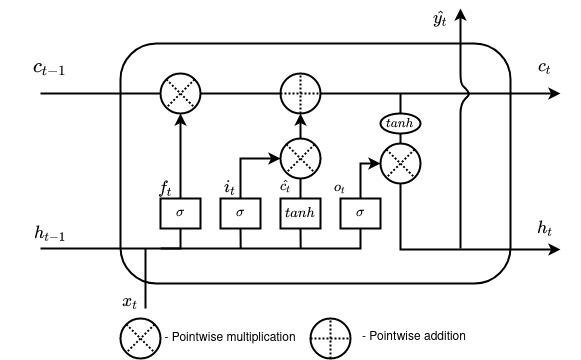
\includegraphics[width=\linewidth]{II_Body/LSTM/images/LSTM.jpg}
    \caption{Long Short-Term Memory Cell}
    \label{fig:LSTM-cell2}
\end{figure}
\begin{equation}
    \begin{split}
        f_t &= \sigma \left(W_f \left[h_{t-1}, x_t \right] + b_f \right) \\
        i_t &= \sigma \left(W_i \left[h_{t-1}, x_t \right] + b_i \right) \\
        o_t &= \sigma \left(W_o \left[h_{t-1}, x_t \right] + b_o \right) \\    
    \end{split}
    \label{eq:LSTM-gates2}
\end{equation}
\begin{equation}
    \begin{split}
        c_t &= f_t c_{t-1}+i_t \times tanh \left(W_c \left[h_{t-1}, x_t \right] + b_c \right) \\
        h_t &= o_t*tanh \left(c_t \right)
    \end{split}
    \label{eq:LSTM-output2}
\end{equation}
}

%
%
The LSTM model has been used widely in stock-price prediction or weather forecasting.
However, unlike State of Charge estimation, which commonly uses $V$, $I$ and $T$ as inputs, those methods utilise the output feature as an input to the subsequent prediction to propagate results further and calculate the time before a critical event occurrence.
Besides, methods like weather forecasting a weak ahead are not limited by lacking output data, since the searched criteria is always known or will be known.
Contrarily, a True State of Charge of a battery cannot be determined and verified against previously made predictions without additional battery modelling techniques. (not to mention of having it integrated into Electric Vehicle.)
(As oppose to the SoC estimate, where getting true values require battery cycler capable with set of ) 
%%%%%%%%%%%
%Unlike the charge estimation, which can only output a single value based on a history of samples, they are not limited to... Therefore does not require the output as input since the truth will become known in due time.

%
%
The best way to utilise the performance of the stateless LSTM model is through training with a data windowing technique.
The NN model will receive a fixed set of equally distributed time samples at each time prediction.
Every next forecast will shift the time window by a constant step $s$, until all possible combinations of time slices go through the model.
That approach is referred to as a stateless model, which sees dependencies over input samples only, rather than preserving every received input, like in stateful implementations.
It also allows the order of the windows to be shuffled to avoid overfitting
Since no dropout was applied before models output a set of strategies strategies has been applied to vary learning rate and rollback before early stopping to assist the fitting process.
\ifthenelse {\boolean{thesis}}
{
Chapter~\ref{} at sections~\ref{}and~\ref{} provide an explanation to those two methods, which already proven to be useful at training SoC models.
} 
{
    \textbf{TODO: EIther import that content from previos article, reference it, or redo entirely}
}
As a result, a NN model will learn dependency between a fixed amount of equally distributed time samples $n$ and yet independent from the order of the inputs.
\mbox{Figure~\ref{fig:Windowing}} demonstrates how the input dataset is constructed and ordered into a 3-dimensional dataset, with 4 features, 500 timestamps and around 110k* samples to fit on.
Due to the size of the windows, equivalent to 8 and quoter minutes of a discharge process, no batching mechanism has been used to reduce computational load and avoid 4-dimensional matrix management.


%
%
The mean and standard deviation has normalised all data to speed up the training process.
The normalisation constant from training input samples must be used for validation and testing sets to ensure the right trends.
The state of charge will be narrowed between 0 and 1 to represent the percentage charge in 2 decimal numbers.
\mbox{Table~\ref{tab:params}} highlights the parameters required to define the initial model, where $s$ defines output step size.
Use of a $\sigma$ function as an output justified by the charge normalisation between 0 and 1.
\begin{table}[ht]
    \renewcommand{\arraystretch}{1.3}
    \caption{Model structure and parameters}
    \centering
    \label{tab:params}
    \resizebox{\columnwidth}{!}{
    \begin{tabular}{ l l l }
        \hline\hline \\[-4mm]
        Input     & $shape= \left( 1,500,4 \right)$ & $batch=1 $  \\
        \hline
        LSTM      & $activation= 'tanh'$ & $units=510$  \\
        \hline
        Dropout   & $0.0$ &   \\
        \hline
        Output    & $activation= \sigma\left(s, 1 \right)$ &   \\
        \hline\hline
    \end{tabular}
    }
\end{table}

%
%
\ifthenelse {\boolean{thesis}}
{
The optimisation algorithm for the fitting process has been defined by regular Adam from the previous chapter, \mbox{Algorithm~\ref{}}, with the corresponding hyperparameters, \mbox{Table~\ref{}}.

}
{
The optimisation algorithm for the fitting process has been defined by Adam, \mbox{Algorithm~\ref{alg:copyAdam}}, with the following hyperparameters, \mbox{Table~\ref{tab:newM-params}}.
%\textcolor{red}{Try to use Robust Adam instead, because why the hell not since I lost one month of my life to implement that cursed algorithm from Javids miss-typed notes? Complete this section with details as per Gareth Javid's implementation if RoAdam will be able to produce a faster fitting.}
\begin{algorithm}\captionsetup{labelfont={sc,bf}, labelsep=newline}
    \caption{Adaptive Moment Estimation (Adam) optimisation}
    \begin{algorithmic}[1]
        \STATE \textbf{Number of input samples} \\ $N\gets length(\textit{input data})$\\
        \STATE \textbf{Size of windows} \\ $S\gets length(V_{i..n})$\\
        \STATE \textbf{Output steps} \\ $O\gets length(V_{i..n})$\\
        \STATE Input: $x_n = [V_{i..n}, I_{i..n}, T_{i..n}, SoC_{(i-1)..(n-1))}]$ \\
         - Shape: $X = (N, S, 4)$
        \STATE Output:$y_n = [SoC_{(n-o)..n}] - $Shape:$Y = (N, O, 1)$
        \STATE Define Loss function: $L$ \\
                Get hyperparameters: $\alpha, \beta_1, \beta_2, \epsilon$
        \WHILE{$W_t \text{ not converge}$}
        \STATE $t \gets t+1$
        \STATE $g_t \gets \nabla_W L_t (W_{t-1})$ \COMMENT{Obtain gradient}
        \STATE $m_t \gets \beta_1 m_{t-1}+(1-\beta_1) g_t $ \COMMENT{$1_{st}$ moment calculation}
        \STATE $\upsilon_t \gets \beta_2 \upsilon_{t-1}+ \left(1-\beta_2 \right)g^2_t $ \COMMENT{$2_{nd}$ moment calculation \label{alg:Adam-Line-2Moment}}
        \STATE $\hat{m_t} \gets \frac{m_t}{1-\beta^t_1}$ \COMMENT{Corrected $\hat{m_t}$}
        \STATE $\hat{\upsilon_t} \gets \frac{\upsilon_t}{1-\beta^t_2} $ \COMMENT{Corrected $\hat{\upsilon_t}$}
        \STATE $W_t \gets W_{t-1}- \alpha \frac{\hat{m_t}}{\sqrt{\hat{\upsilon_t}}+\epsilon} $ \COMMENT{Update parameters}
        \ENDWHILE
    \end{algorithmic}
    \label{alg:copyAdam}
\end{algorithm}
\begin{table}[htbp]
    \renewcommand{\arraystretch}{1.3}
    \caption{Optimiser specific hyperparameters}
    \centering
    \label{tab:newM-params}
    \resizebox{\columnwidth}{!}{
    \begin{tabular}{ l l l l }
        \hline\hline \\[-4mm]
        $\alpha$ & $\beta_1 $ & $\beta_2$ & $\epsilon$ \\
        \hline
        $0.001$ & $0.9$ & $0.999$ & $10^{-8}$ \\% 0.0000001
        \hline\hline
    \end{tabular}
    }
\end{table}
}  
\subsection{Development of Feed-Forward Autoregressive model} \label{sec:feed}
  The regular training procedure for a 4-feature model has a significant limitation. The model does not consider the Feed-Forward application of the prediction output.
In the case of excellent input values, the output is expected to be within~1 \% miss-accuracy since from 500 ideal SoC values, estimation of value 501 is a trivial task.

%
%
Two subplots, \mbox{Figure~\ref{fig:regular_tr}}, demonstrate the prediction results of a four-feature-based FUDS-trained simple LSTM model against a single battery cycle of DST driving.
\mbox{Figure~\ref{fig:regular_tr}a} demonstrates the prediction with input SoC based on known perfect State of Charge at any random point in time, marked with a red dotted line (i.e. 500 values for SoC, with sensory data, from learning used to predict charge at 501).
On the other hand, the \mbox{Figure~\ref{fig:regular_tr}b} uses the feedforward approach, where only the first sample window has the true SoC.
Every upcoming prediction replaces the known value with a prediction and therefore has a strict order of samples from start to end, marked as a yellow dotted line.
The same colour annotation will be used for all the remaining plots to distinguish the input schemes.
\ifthenelse{\boolean{thesis}}{
    \begin{figure}[htbp]
        \centering
        % DST based tests
        \begin{subfigure}[b]{0.485\textwidth}
            \centering
            % \includesvg[width=\linewidth]{III_Conclussion/im_compare/FUDS-val-48.svg}
            \includesvg[width=\linewidth]{III_Conclussion/im_compare/SMFUDS-val-9.svg}
            \caption{Regular training process snapshot}
            \label{subfig:regular_tr}
        \end{subfigure}
        \hfill
        \begin{subfigure}[b]{0.485\textwidth}
            \centering
            \includesvg[width=\linewidth]{III_Conclussion/im_compare/SMFUDS-FF-9.svg}
            \caption{Feed-Forward validation process snapshot}
            \label{subfig:regular_ts}
        \end{subfigure}
        \caption{Comparison between training and testing accuracies of a 4-featured based model with a default training and testing loop.}
        \label{fig:regular_tr}
    \end{figure}
} {
    \begin{figure*}[!t]
        \centering
        % DST based tests
        \subfloat[Regular training process snapshot]{\includesvg[width=0.485\linewidth]{III_Conclussion/im_compare/SMFUDS-val-9.svg}}
        \hfill
        \subfloat[Feed-Forward validation process snapshot]{\includesvg[width=0.485\linewidth]{III_Conclussion/im_compare/SMFUDS-FF-9.svg}}
        \caption{Comparison between training and testing accuracies of a 4-featured based model with a default training and testing loop.}
        \label{fig:regular_tr}
    \end{figure*}
}

%
%
%
The green error area axis has been dropped from \mbox{Figure~\ref{fig:regular_tr}b} due to high inaccuracy, which would cover half of the plot area.
\ifthenelse{\boolean{thesis}}{The implementation of this prediction method is presented in \mbox{Appendix~\ref{app:Feed-Forward}}.}{}
It demonstrates how the appended charge output model accumulates the error with every dependent input in a single prediction.
If that output is used for further prediction and the model keeps preserving the dependency, the miss accuracy value rises non-linearly.
This is a good justification for why there has been no evidence in the published literature of utilising a feed-forward approach to the SoC estimation.

%
%
%! Get eid of that figgure, find a way to refer to it.
The reason for that lies in the weights the model places on the State of Charge input feature.
For a better weight balance, the training procedure must be modified to consider the possibility of an inaccuracy in the input charge data.
One example of a modified training loop are Autoregressive models~\cite{time_2020}.
The implementation can be applied to any early-created model, referring to regressive implementation.
However, this is an example of the earlier mentioned stateful data management, where the model was explicitly programmed to run internally automatically and remains of stateless type.
The state will be produced and used internally but is not present in the outputs.
\ifthenelse{\boolean{thesis}}{\mbox{Figure~\ref{fig:autoregressive}} demonstrate how a trained model internally uses produced prediction to produce more than a single output ahead of time.
For example, from a given input of sensory data of 23 days, a weather prediction model estimates a further three weeks ahead.
However, this case produces the exact number of output features, matching the input to make the prediction work properly.
Besides, once the 24 day comes, the same model can be updated with new actual information, adjusting the follow-up for three weeks.
In the case of the State of Charge prediction model, such an approach cannot be used by itself since the SoC can not be determined like sensory data.
\begin{figure}[ht]
    \centering
    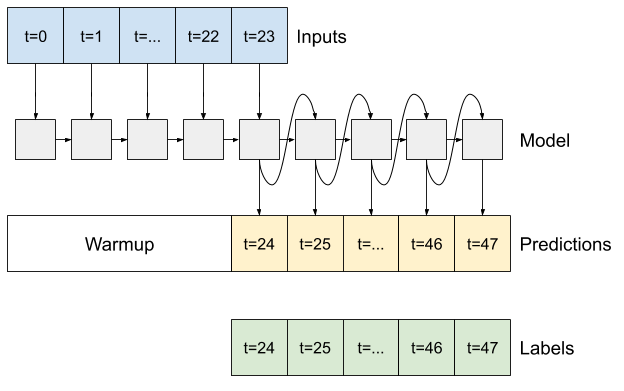
\includegraphics[width=\columnwidth]{II_Body/images/multistep_autoregressive.png}
    \caption{Autoregressive model input and output demonstration from time-series tutorial~\cite{time_2020}}
    \label{fig:autoregressive}
\end{figure}
} {The implementation demonstration from time-series tutorial~\cite{time_2020} of the utilised Machine Learning framework provides both a written and visual explanation of Autoregression implementation in the context of weather prediction ahead of time.
In the case of the State of Charge prediction model, such an approach cannot be used by itself since the SoC can not be determined like sensory data.
Therefore, it will be adapted to overcome the problem of accumulated error in the feed-forward estimation method.}

%
%
\ifthenelse{\boolean{thesis}}{The SoC estimation model may benefit from multiple outputs by adapting the Autoregression to the accumulator utilisation scenario.
Therefore, the}
{The} training procedure for the regular LSTM model has been modified to consider potential inaccuracy in the known data rather than the future outputs.
The diagram in Figure~\ref{fig:training_testing} illustrates how the technique has been adapted to the current research.
\ifthenelse{\boolean{thesis}}{Unlike Figure~\ref{fig:autoregressive}, the training and testing procedures were separated from each other on two separate subfigures.}
{Unlike with Autoregressive example from the documentation tutorial~\cite{time_2020}, the training and testing procedures were separated from each other on two separate subfigures.}
% The diagram in \mbox{Figure~\ref{subfig:testing}} illustrates regular training and testing procedures for a model to produce output.
The diagram in \mbox{Figure~\ref{fig:training_testing}a} demonstrates the procedure for the model call using autoregression during the training, whereas \mbox{Figure~\ref{fig:training_testing}b} only shows as a comparison to the regular usage and during the actual application or testing.
\ifthenelse{\boolean{thesis}}{Code-based detailed implementation have been attached in Appendix~\ref{app:AutoFeedback}.}{}
% Unlike regular LSTM, training and testing differ from each other.
If the testing procedure remains unchanged, the training performs multiple calls during a single-window sample processing.
Every new call outputs the results and feeds again into the same model, with one sample from each sensor.
Each output also contained a model state, containing the values stored in the cells, preserving dependency between model calls.
% State output is used only for internal model processing.
Every output of every step has been stored in the returned array for the optimiser to adjust weights.
With a new approach, it will compare an array of predicted samples against the actual values of the SoC, making the adjustments based on the inaccuracies present in the dependencies and considering them as part of the system.
Unlike testing, the training is not feed-forward based; therefore, all actual SoC data and known SoC inputs are considered true, except the last $s$, which matches the number of outputs.
% This was meant to increase the model fit process.
The more output samples the model returns during the training (Returned training array), the longer the training process becomes, but the better the real-time prediction against aggressive driving profiles gets achieved.
\ifthenelse{\boolean{thesis}}{
    \begin{figure}[htbp]
        \centering
        % DST based tests
        \begin{subfigure}[b]{0.85\textwidth}
            \centering
            % 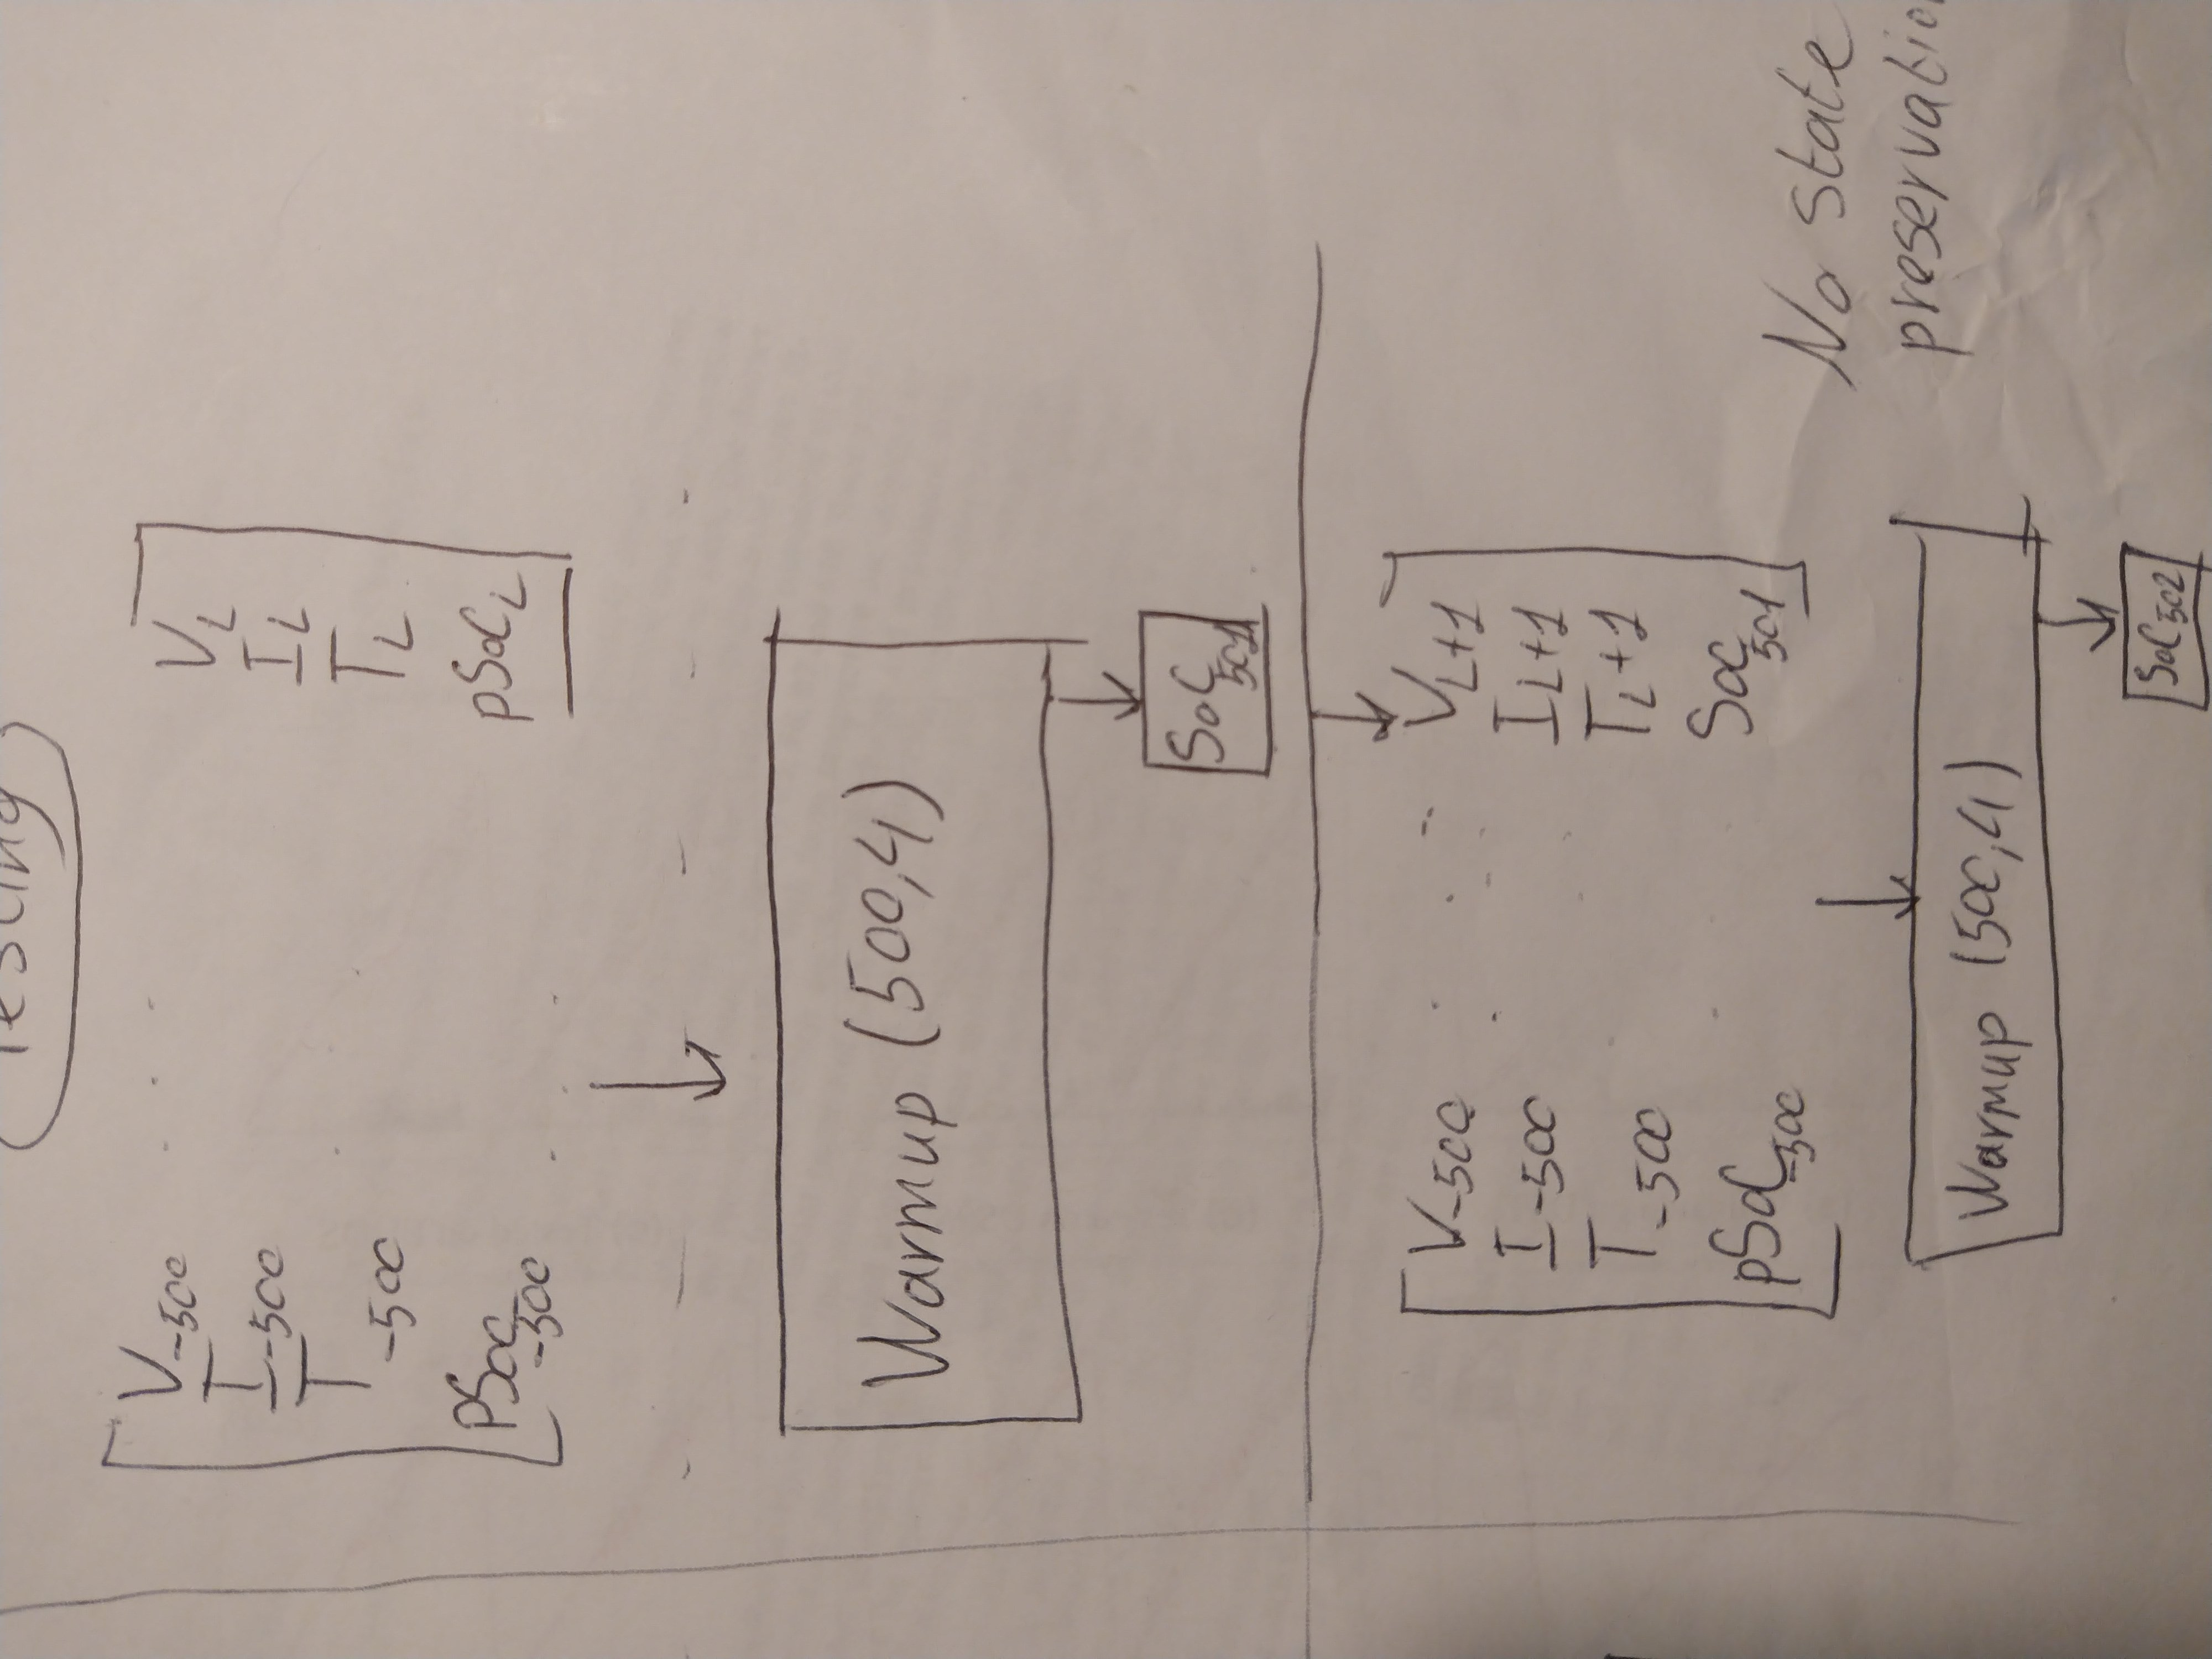
\includegraphics[width=\linewidth]{II_Body/images/IMG_20210524_133103.jpg}
            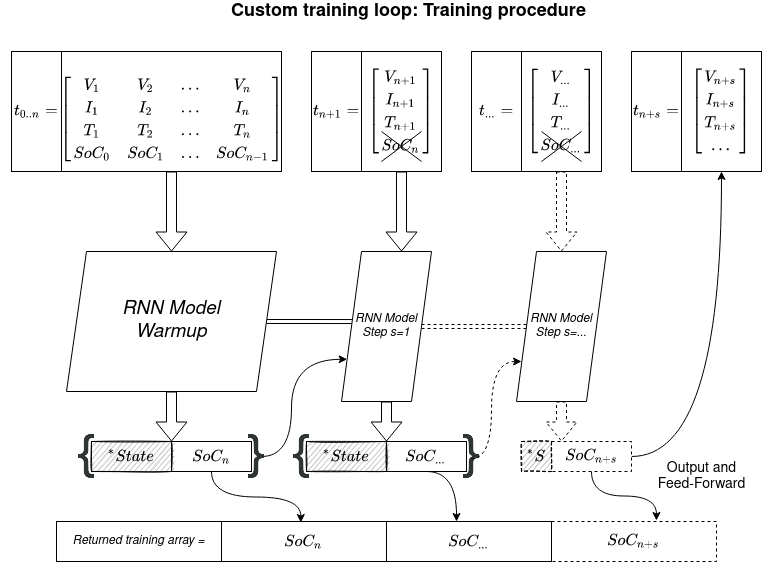
\includegraphics[width=\linewidth]{II_Body/images/Autoregression-Training.png}
            \caption{Custom autoregressive training procedure}
            \label{subfig:training}
        \end{subfigure}
        \hfill
        \begin{subfigure}[b]{0.85\textwidth}
            \centering
            % 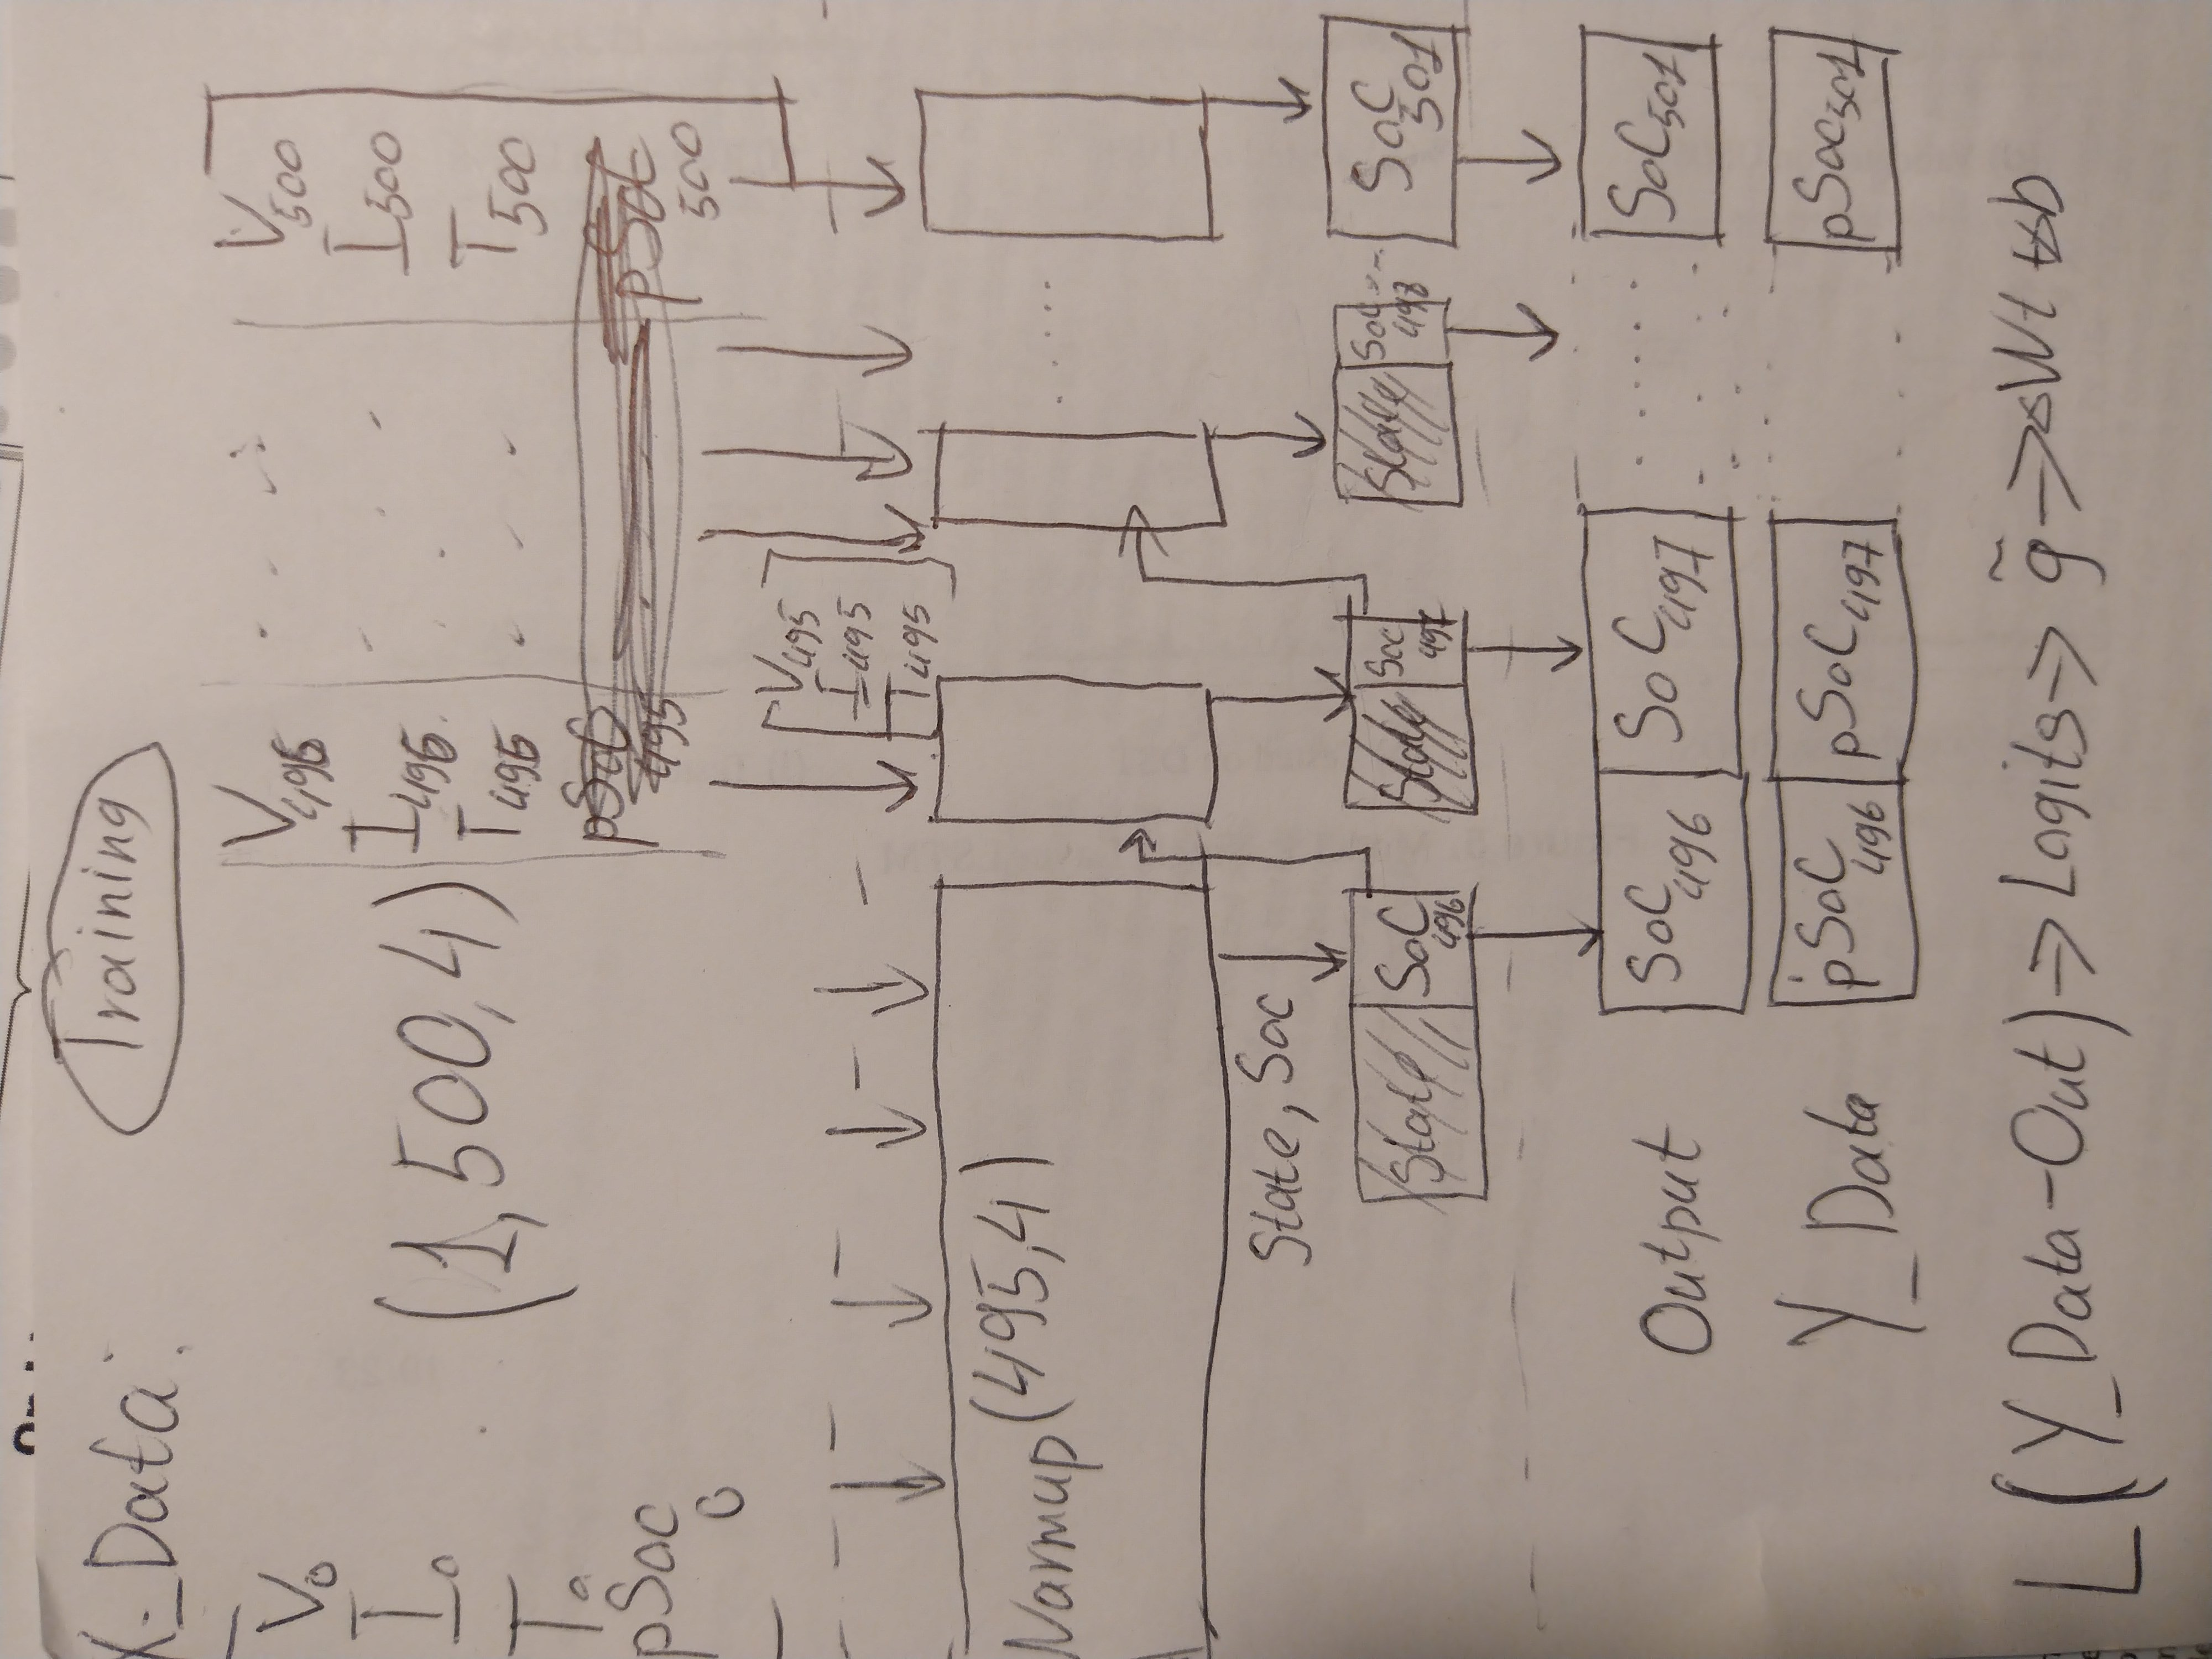
\includegraphics[width=\linewidth]{II_Body/images/IMG_20210524_133052.jpg}
            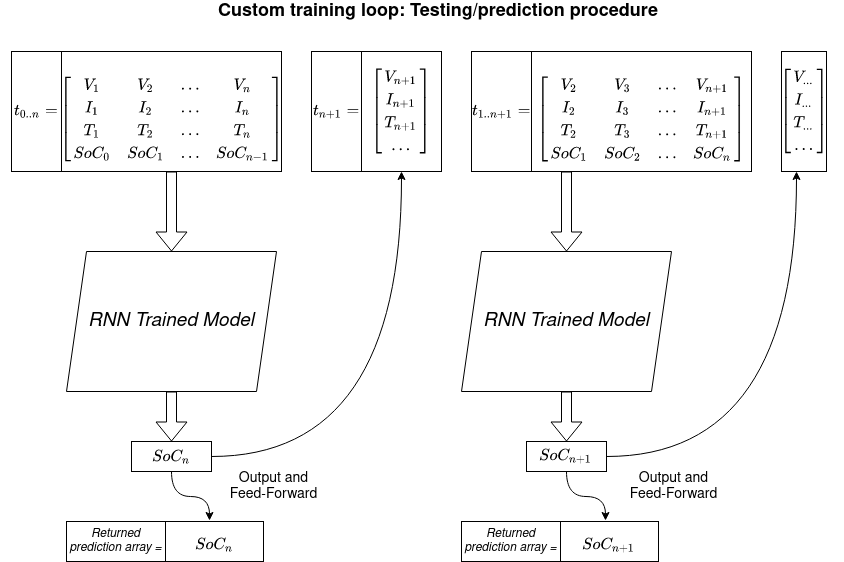
\includegraphics[width=\linewidth]{II_Body/images/Autoregression-Testing.png}
            \caption{Regular testing and validation procedure}
            \label{subfig:testing}
        \end{subfigure}
        \caption{Block diagram demonstration of training and testing working procedures for 4-featured-based models.}
        \label{fig:training_testing}
    \end{figure}
} {
    % \begin{figure*}[!t]
    %     \centering
    %     % DST based tests
    %     \subfloat[Custom autoregressive training procedure]{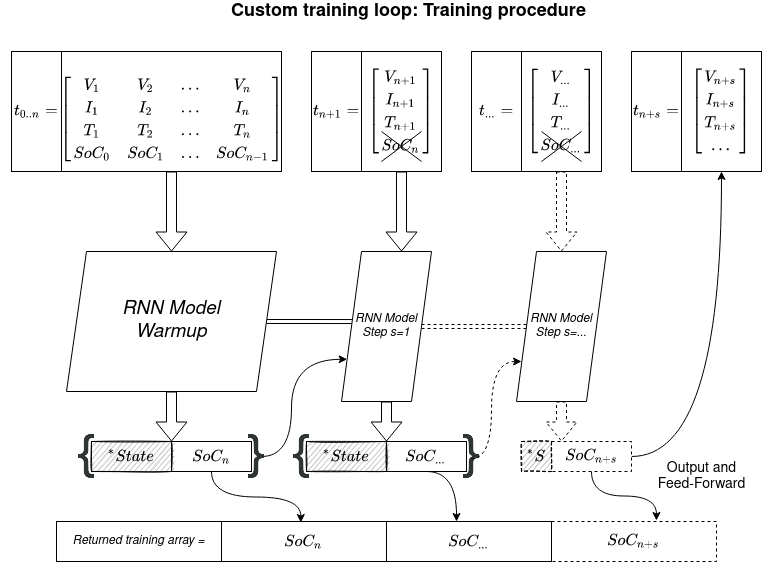
\includegraphics[width=0.85\linewidth]{II_Body/images/Autoregression-Training.png}}
    %     \hfill
    %     \subfloat[Regular testing and validation procedure]{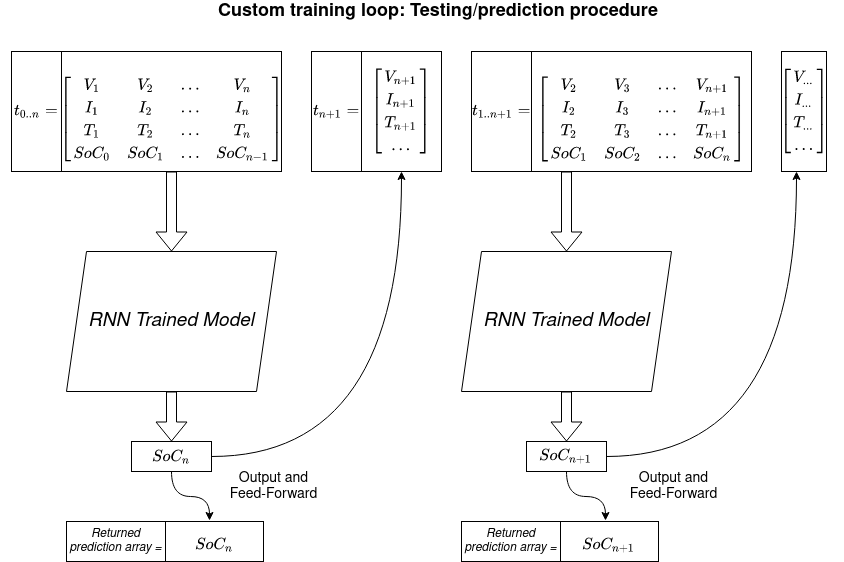
\includegraphics[width=0.85\linewidth]{II_Body/images/Autoregression-Testing.png}}
    %     \caption{Block diagram demonstration of training and testing working procedures for 4-featured-based models.}
    %     \label{fig:training_testing}
    % \end{figure*}
    \begin{figure*}[!t]
        \centering
        % DST based tests
        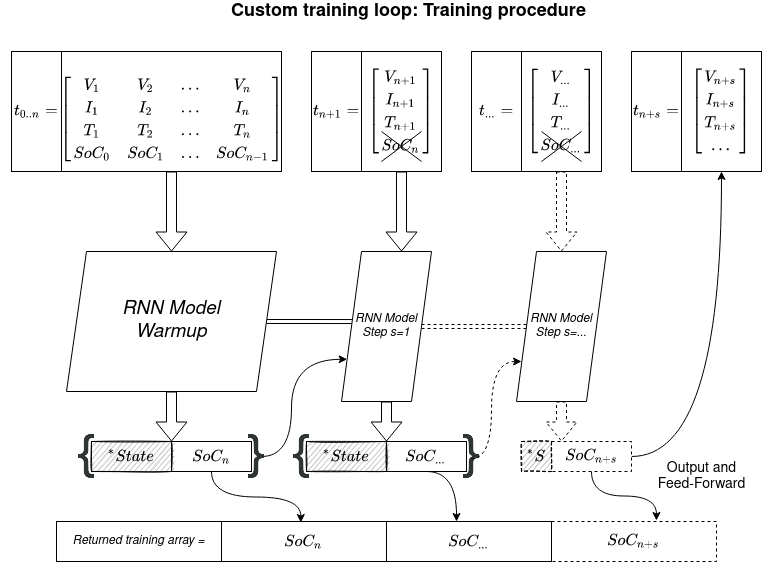
\includegraphics[width=0.85\linewidth]{II_Body/images/Autoregression-Training.png}
        \caption{Block diagram demonstration of custom autoregressive training procedure for 4-featured-based models.}
        \label{fig:training_testing}
    \end{figure*}
}

%
%
Now, with modified training procedure and optimiser usage of the 30 output samples (29 known and one predicted) as an example, \mbox{Figure~\ref{fig:modefied_tr}} contains a similar test, as without autoregression on earlier Figure~\ref{fig:regular_tr}.
Even though the accuracy with tabled samples has decreased between \mbox{Figure~\ref{fig:regular_tr}a and~\ref{fig:modefied_tr}a}, its feed-forward prediction accuracy has significantly increased and does not lose the trend, \mbox{Figure~\ref{fig:regular_tr}b and~\ref{fig:modefied_tr}b}.
The implementation has been based on contributions from the original framework developers~\cite{time_2020} and written based on corresponding original documentation of Tensorflow 2.3~\cite{tensorflow2015-whitepaper}.
\ifthenelse{\boolean{thesis}}{
\begin{figure}[H]
    \centering
    \begin{subfigure}[b]{0.485\textwidth}
        \centering
        % \includesvg[width=\linewidth]{III_Conclussion/Models/Sadykov2021-30steps/FUDS-models/SMRFUDSval-19.svg}
        \includesvg[width=\linewidth]{III_Conclussion/im_compare/SMRFUDSval-19.svg}
        \caption{Modified training process}
        \label{subfig:modefied_tr}
    \end{subfigure}
    \begin{subfigure}[b]{0.485\textwidth}
        \centering
        % \includesvg[width=\linewidth]{III_Conclussion/Models/Sadykov2021-30steps/FUDS-models/SMRFUDS-FF-19.svg}
        \includesvg[width=\linewidth]{III_Conclussion/im_compare/SMRFUDS-FF-19.svg}
        \caption{Feed-Forward validation process}
        \label{subfig:modefied_ts}
    \end{subfigure}
    \caption{Comparison between training and testing accuracies of a 4-featured based model with a modified training and default testing loops.}
    \label{fig:modefied_tr}
\end{figure}
} {
\begin{figure*}[!t]
    \centering
    \subfloat[Modified training process]{\includesvg[width=0.485\linewidth]{III_Conclussion/im_compare/SMRFUDSval-19.svg}}
    \label{subfig:modefied_tr}
    \subfloat[Feed-Forward validation process]{\includesvg[width=0.485\linewidth]{III_Conclussion/im_compare/SMRFUDS-FF-19.svg}}
    \label{subfig:modefied_ts}
    \caption{Comparison between training and testing accuracies of a 4-featured based model with a modified training and default testing loops.}
    \label{fig:modefied_tr}
\end{figure*}
}

\newpage

\section{Results} \label{sec:results}
\ifthenelse{\boolean{thesis}}{
An optimal set of hyperparameters has been obtained based on early results in Chapter~\ref{cha:Analysis}, Section~\ref{sec:AN:Results}.
} {
An optimal set of hyperparameters has been obtained based on early results in previous work~\cite{sadykov_practical_2022}.
}
However, the number of outputs from a model, referred to as output steps, had to be experimentally tested and compared prior to the primary training procedure.
After that, ten models of a single layer with 131 neurons of LSTM with Autoregression were trained on all provided temperature ranges ten times, validated against 25\textdegree{}C of its' profile, and tested against 25 \& 30\textdegree{}C of the other two profiles.
An average of all ten results were plotted and later tested against the entire training sets to measure the performance and minimise the stochastic effect.

\subsection{Optimal output step size}
    The optimal size of the Autoregression output steps $AR_{width}$ for better capturing the SoC was determined through experimental training.
    \mbox{Table~\ref{tab:out_steps}} outlines the training iterations of each driving profile until it reaches accuracy below 2.5\%
    \ifthenelse{\boolean{thesis}}{, and Figure~\ref{fig:Models_res} plots the final best results on a feed-forward test. } {.}
    % The training continued for as long as there was no overfitting determined.
    During $AR_{width}$ evaluation through several attempts, no overfitting has been observed in testing to date.
    Profiles which already reached an error below the predetermined error were excluded from the follow up experiments.
    Those that did not reach 2.5\% were prevented from more epoch training since the increase of $AR_{width}$ by five more samples is more time convenient than waiting for the error to diverge.
    Because of that, even with 25 steps on FUDS dataset providing a reasonable accuracy, the increase towards 30 lowered the percentage below the initially expected and achieved it through fewer epochs.
    \ifthenelse{\boolean{thesis}}{
    \begin{table}[htbp]
        \renewcommand{\arraystretch}{1.3}
        \caption{Percentage accuracy evaluation with increasing output step size}
        \centering
        \label{tab:out_steps}
        \begin{tabular}{ c | c c c | r }
            \hline\hline \\[-4mm]
            $AR_{width}$ & DST & US06 & FUDS & Epochs \\
            \hline
            10 & 2.94 & $\geq\sim 15$ & $\geq\sim 15$ & 8 \\
            15 & 0.90 & 10.67 & 11.10 & 8 \\
            20 & -- & 0.68  &  4.25 & 10 \\
            25 & -- & --  &  3.48 & 25 \\
            30 & -- & --  &  0.59 & 19 \\
            \hline\hline
        \end{tabular}
    \end{table}
    }{
    \begin{table}[htbp]
        \renewcommand{\arraystretch}{1.3}
        \caption{Percentage accuracy evaluation with increasing output step size}
        \centering
        \label{tab:out_steps}
        \resizebox{\columnwidth}{!}{
        \begin{tabular}{ c | c c c | r }
            \hline\hline \\[-4mm]
            $AR_{width}$ & DST & US06 & FUDS & Epochs \\
            \hline
            10 & 2.94 & $\geq\sim 15$ & $\geq\sim 15$ & 8 \\
            15 & 0.90 & 10.67 & 11.10 & 8 \\
            20 & -- & 0.68  &  4.25 & 10 \\
            25 & -- & --  &  3.48 & 25 \\
            30 & -- & --  &  0.59 & 19 \\
            \hline\hline
        \end{tabular}
        }
    \end{table}
    }
    
%
%
\ifthenelse{\boolean{thesis}}{
The Dynamic Stress Test has a stable trend of current consumption and regenerative process.
Therefore it did not take long to capture the behaviour of the charge.
A single cycle on \mbox{subfigure~\ref{subfig:res_DST}} provides an example of accurate feed-forward charge estimation with output steps between 10-15 samples.
The US06 and FUDS have more aggressive current usage, leading to a higher step $s$ number.
As per \mbox{subfigures~\ref{subfig:res_US} and~\ref{subfig:res_FUDS}}, it took twice as many output samples to achieve similar accuracy to the DST-based model.
Any further increase can capture even more complicated scenarios, leading to a longer training time.
However, every added step decreased the epoch per training model to produce the best fit.
\begin{figure}[htbp]
    \centering
    % DST based tests
    \begin{subfigure}[b]{0.325\textwidth}
        \centering
        % \includesvg[width=\linewidth]{III_Conclussion/Models/Sadykov2021-15steps/DST-models/SMRDST-FF-8.svg}
        \includesvg[width=\linewidth]{III_Conclussion/im_steps/SMRDST-FF-8.svg}
        \caption{Best DST based model after 8 iterations with 15 steps}
        \label{subfig:res_DST}
    \end{subfigure}
    \hfill
    \begin{subfigure}[b]{0.325\textwidth}
        \centering
        % \includesvg[width=\linewidth]{III_Conclussion/Models/Sadykov2021-20steps/US06-models/SMRUS06-FF-10.svg}
        \includesvg[width=\linewidth]{III_Conclussion/im_steps/SMRUS06-FF-10.svg}
        \caption{Best US06 based model after 10 iterations with 20 steps}
        \label{subfig:res_US}
    \end{subfigure}
    \hfill
    \begin{subfigure}[b]{0.325\textwidth}
        \centering
        % \includesvg[width=\linewidth]{III_Conclussion/im_best/FUDS-19.svg}
        % \includesvg[width=\linewidth]{III_Conclussion/Models/Sadykov2021-30steps/FUDS-models/SMRFUDS-FF-19.svg}
        \includesvg[width=\linewidth]{III_Conclussion/im_steps/SMRFUDS-FF-19.svg}
        \caption{Best FUDS based model after 19 iterations with 30 steps}
        \label{subfig:res_FUDS}
    \end{subfigure}
    \caption{Best training results over 3 different driving profiles}
    \label{fig:Models_res}
\end{figure}
%
%
An optimal step is required for running the training process on the entire dataset with all three profiles as inputs to prepare for future deployment on hardware.
Therefore, all other results demonstrations will use 30 steps as the most optimal and report any other results based on that parameter.
} { 
Because all drive cycles were suitably accurate after 30 steps of $AR_{width}$,
the same value will be used for all further models.
Despite making the training process slow compared to other steps due to concurrent looping through additional outputs and feed-forward, the time for producing a single sample at the output is the same.
}

\subsection{Accuracy comparison}
With cross-training and testing over ten attempts average (to minimise the stochastic nature of the Machine Learning), Figure~\ref{fig:Model-6res} has been produced to demonstrate the resulting predictions.
The total errors for each model are summarised in Table~\ref{tab:acc-results2}.
It shows results from the most accurate model in~\cite{sadykov_practical_2022}, model 1 \& 3, compared to present results.
In total, 30 models were produced in this study, averaged, and compared for the best usage in an Electric Vehicle.
\ifthenelse{\boolean{thesis}}{
\begin{figure*}[htbp]
    \centering
    %%%%%%%%%%%%%%%%% DST based tests %%%%%%%%%%%%%%%%%
    \begin{subfigure}[b]{0.325\textwidth}
        \centering
        \includesvg[width=\linewidth]{II_Body/images/M6-history-DST-mae.svg}
        \caption{Average training and testing MAE history average of 10 attempts}
    \end{subfigure}
    \hfill
    \begin{subfigure}[b]{0.325\textwidth}
        \centering
        \includesvg[width=\linewidth]{II_Body/images/DST-6-train.svg}
        \caption{Validation on a single DST cycle of SoC estimation average of 10 attempts at 25\textdegree{}C}
    \end{subfigure}
    \hfill
    \begin{subfigure}[b]{0.325\textwidth}
        \centering
        \includesvg[width=\linewidth]{II_Body/images/DST-6-test.svg}
        \caption{Testing on two cycles of US06 and FUDS profiles average of 10 attempts}
        \label{subfig:Model-6res-DSTvsFUDS}
    \end{subfigure}
    %%%%%%%%%%%%%%%%% US06 based tests %%%%%%%%%%%%%%%%%
    \begin{subfigure}[b]{0.325\textwidth}
        \centering
        \includesvg[width=\linewidth]{II_Body/images/M6-history-US06-mae.svg}
        \caption{Average training and testing MAE history average of 10 attempts}
    \end{subfigure}
    \hfill
    \begin{subfigure}[b]{0.325\textwidth}
        \centering
        \includesvg[width=\linewidth]{II_Body/images/US06-6-train.svg}
        \caption{Validation on a single US06 cycle of SoC estimation average of 10 attempts at 25\textdegree{}C}
    \end{subfigure}
    \hfill
    \begin{subfigure}[b]{0.325\textwidth}
        \centering
        \includesvg[width=\linewidth]{II_Body/images/US06-6-test.svg}
        \caption{Testing on two cycles of DST and FUDS profiles average of 10 attempts}
    \end{subfigure}
    % %%%%%%%%%%%%%%%%% FUDS based tests %%%%%%%%%%%%%%%%%
    \begin{subfigure}[b]{0.325\textwidth}
        \centering
        \includesvg[width=\linewidth]{II_Body/images/M6-history-FUDS-mae.svg}
        \caption{Average training and testing MAE history average of 10 attempts}
    \end{subfigure}
    \hfill
    \begin{subfigure}[b]{0.325\textwidth}
        \centering
        \includesvg[width=\linewidth]{II_Body/images/FUDS-6-train.svg}
        \caption{Validation on a single FUDS cycle of SoC estimation average of 10 attempts at 25\textdegree{}C}
    \end{subfigure}
    \hfill
    \begin{subfigure}[b]{0.325\textwidth}
        \centering
        \includesvg[width=\linewidth]{II_Body/images/FUDS-6-test.svg}
        \caption{Testing on two cycles of DST and US06 profiles average of 10 attempts}
    \end{subfigure}
    \caption{Model 6: Stateless LSTM with 30 steps of Autoregression.}
    \label{fig:Model-6res}
\end{figure*}
} {
\begin{figure*}[!h]
    \centering
    %%%%%%%%%%%%%%%%% DST based tests %%%%%%%%%%%%%%%%%
    \subfloat[Average training and testing MAE history; average of 10 attempts]{\includesvg[width=0.325\linewidth]{II_Body/images/M6-history-DST-mae.svg}}
    \hfill
    \subfloat[Validation on a single DST cycle of SoC estimation; average of 10 attempts at 25\textdegree{}C]{\includesvg[width=0.325\linewidth]{II_Body/images/DST-6-train.svg}}
    \hfill
    \subfloat[Testing on two cycles of US06 and FUDS profiles; average of 10 attempts]{\includesvg[width=0.325\linewidth]{II_Body/images/DST-6-test.svg}}
    \label{subfig:Model-6res-DSTvsFUDS}
    %%%%%%%%%%%%%%%%% US06 based tests %%%%%%%%%%%%%%%%%
    \subfloat[Average training and testing MAE history; average of 10 attempts]{\includesvg[width=0.325\linewidth]{II_Body/images/M6-history-US06-mae.svg}}
    \hfill
    \subfloat[Validation on a single US06 cycle of SoC estimation; average of 10 attempts at 25\textdegree{}C]{\includesvg[width=0.325\linewidth]{II_Body/images/US06-6-train.svg}}
    \subfloat[Testing on two cycles of DST and FUDS profiles; average of 10 attempts]{\includesvg[width=0.325\linewidth]{II_Body/images/US06-6-test.svg}}
    % %%%%%%%%%%%%%%%%% FUDS based tests %%%%%%%%%%%%%%%%%
    \hfill
    \subfloat[Average training and testing MAE history; average of 10 attempts]{\includesvg[width=0.325\linewidth]{II_Body/images/M6-history-FUDS-mae.svg}}
    \hfill
    \subfloat[Validation on a single FUDS cycle of SoC estimation; average of 10 attempts at 25\textdegree{}C]{\includesvg[width=0.325\linewidth]{II_Body/images/FUDS-6-train.svg}}
    \hfill
    \subfloat[Testing on two cycles of DST and US06 profiles; average of 10 attempts]{\includesvg[width=0.325\linewidth]{II_Body/images/FUDS-6-test.svg}}
    \caption{Model 6: Stateless LSTM with 30 steps of Autoregression.}
    \label{fig:Model-6res}
\end{figure*}
}
\ifthenelse {\boolean{thesis}}
{
\begin{table}[htbp]
    \renewcommand{\arraystretch}{1.3}
    \caption{Accuracy result summary for entire training datasets between best existing models from Chapter~\ref{cha:Analysis} and novel method.}
    \centering
    \label{tab:acc-results2}
\resizebox{\textwidth}{!}{
\begin{tabular}{ c| l| c c c| c c c |c c c}
    \hline\hline \\[-4mm]
% Columns setup
    \multirow{3}{1em}{\#} &
    \multirow{3}{3em}{Trained} &
    \multicolumn{9}{c}{Tested} \\
    \cline{3-11}
    & & 
    \multicolumn{3}{c|}{DST} &
    \multicolumn{3}{c|}{US06} &
    \multicolumn{3}{c}{FUDS} \\
    \cline{3-11}
     & & MAE(\%) & RMSE(\%) & $R^{2}$(\%) & MAE(\%) & RMSE(\%) & $R^{2}$(\%) & MAE(\%) & RMSE(\%) & $R^{2}$(\%) \\
     \hline
     \textbf{New} & \textbf{DST} & \textbf{0.81} & \textbf{1.10} & \textbf{99.87} & \textbf{1.92} & \textbf{2.71} & \textbf{99.21} & \textbf{1.77} & \textbf{2.35} & \textbf{99.40}  \\
     \textbf{Met-}& \textbf{US06} & \textbf{1.49} & \textbf{2.02} & \textbf{99.57} & \textbf{0.89} & \textbf{1.06} & \textbf{99.88} & \textbf{1.28} & \textbf{1.94} & \textbf{99.59}  \\
     \textbf{hod} & \textbf{FUDS} & \textbf{2.10} & \textbf{2.94} & \textbf{99.10} & \textbf{1.28} & \textbf{1.87} & \textbf{99.62} & \textbf{0.50} & \textbf{0.68} & \textbf{99.95}  \\
    \hline
    % Content
    %Chemali2017
      & DST & 2.77 & 3.52 & 98.71 & 2.86 & 3.93 & 98.34 & 3.28 & 4.62 & 97.66 \\ 
    1 & US06 & 5.97 & 7.97 & 93.39 & 3.37 & 4.14 & 98.15 & 5.38 & 6.93 & 94.73 \\ 
      & FUDS & 5.03 & 7.26 & 94.51 & 4.02 & 6.07 & 96.04 & 1.95 & 2.85 & 99.11 \\ 
    \hline
      & DST & 2.86 & 3.60 & 98.65 & 2.91 & 3.79 & 98.46 & 3.73 & 5.18 & 97.06 \\ 
    3 & US06 & 5.98 & 8.26 & 92.90 & 3.35 & 4.11 & 98.19 & 5.27 & 6.84 & 94.87 \\ 
      & FUDS & 5.33 & 7.25 & 94.53 & 3.61 & 5.53 & 96.71 & 1.82 & 2.51 & 99.31 \\ 
    % GelarehJavid2020
    % \hline
    %   & DST & 2.89 & 3.61 & 98.65 & 3.82 & 5.38 & 96.88 & 4.11 & 5.51 & 96.67 \\ 
    % 4 & US06 & 6.19 & 8.57 & 92.35 & 3.30 & 4.12 & 98.17 & 5.42 & 6.82 & 94.91 \\ 
    %   & FUDS & 5.74 & 7.49 & 94.16 & 4.03 & 5.75 & 96.44 & 1.58 & 2.28 & 99.43 \\ 
    \hline\hline
\end{tabular}
}
\end{table}
} {
\begin{table*}[!ht]
    \renewcommand{\arraystretch}{1.3}
    \caption{Accuracy result summary for entire training datasets. 
    Models 1 and 3 were taken from previous work~\cite{sadykov_practical_2022}.}
    \centering
    \label{tab:acc-results2}
\resizebox{\linewidth}{!}{
    \begin{tabular}{ c l c c c c c c c c c}
        \hline\hline \\[-4mm]
    % Columns setup
        \multirow{4}{*}{\textbf{\#}\vspace{+8pt}} &
        \multirow{4}{*}{\textbf{Trained}\vspace{+8pt}} &
        \multicolumn{9}{c}{\textbf{Tested}} \\
        \cline{3-11}
        & & 
        \multicolumn{3}{c}{\textbf{DST}} &
        \multicolumn{3}{c}{\textbf{US06}} &
        \multicolumn{3}{c}{\textbf{FUDS}} \\
        \cline{3-11}
        & & \textbf{MAE~(\%)} & \textbf{RMSE~(\%)} & \textbf{\boldmath{$R^{2}$~(\%)}} & \textbf{MAE~(\%)} & \textbf{RMSE~(\%)} & \textbf{\boldmath{$R^{2}$~(\%)}} & \textbf{MAE~(\%)} & \textbf{RMSE~(\%)} & \textbf{\boldmath{$R^{2}$~(\%)}} \\
    \hline
        \textbf{New} & \textbf{DST} & \textbf{0.81} & \textbf{1.10} & \textbf{99.87} & \textbf{1.92} & \textbf{2.71} & \textbf{99.21} & \textbf{1.77} & \textbf{2.35} & \textbf{99.40}  \\
        \textbf{Met-}& \textbf{US06} & \textbf{1.49} & \textbf{2.02} & \textbf{99.57} & \textbf{0.89} & \textbf{1.06} & \textbf{99.88} & \textbf{1.28} & \textbf{1.94} & \textbf{99.59}  \\
        \textbf{hod} & \textbf{FUDS} & \textbf{2.10} & \textbf{2.94} & \textbf{99.10} & \textbf{1.28} & \textbf{1.87} & \textbf{99.62} & \textbf{0.50} & \textbf{0.68} & \textbf{99.95}  \\
    \hline
    % Content
    %Chemali2017
        & DST & 2.77 & 3.52 & 98.71 & 2.86 & 3.93 & 98.34 & 3.28 & 4.62 & 97.66 \\ 
    1~\cite{sadykov_practical_2022} & US06 & 5.97 & 7.97 & 93.39 & 3.37 & 4.14 & 98.15 & 5.38 & 6.93 & 94.73 \\ 
        & FUDS & 5.03 & 7.26 & 94.51 & 4.02 & 6.07 & 96.04 & 1.95 & 2.85 & 99.11 \\ 
    \hline
        & DST & 2.86 & 3.60 & 98.65 & 2.91 & 3.79 & 98.46 & 3.73 & 5.18 & 97.06 \\ 
    3~\cite{sadykov_practical_2022} & US06 & 5.98 & 8.26 & 92.90 & 3.35 & 4.11 & 98.19 & 5.27 & 6.84 & 94.87 \\ 
        & FUDS & 5.33 & 7.25 & 94.53 & 3.61 & 5.53 & 96.71 & 1.82 & 2.51 & 99.31 \\ 
    % GelarehJavid2020
    % \hline
    %   & DST & 2.89 & 3.61 & 98.65 & 3.82 & 5.38 & 96.88 & 4.11 & 5.51 & 96.67 \\ 
    % 4 & US06 & 6.19 & 8.57 & 92.35 & 3.30 & 4.12 & 98.17 & 5.42 & 6.82 & 94.91 \\ 
    %   & FUDS & 5.74 & 7.49 & 94.16 & 4.03 & 5.75 & 96.44 & 1.58 & 2.28 & 99.43 \\ 
    \hline\hline
\end{tabular}
}
\end{table*}
}

%!
%!
% \textcolor{red}{Explanation for variance plot is missing. Jump to Pr Lovel discussion at 55:00 for Fig~\ref{fig:Models-var}}
% For a better performance comparison, the variance plot on Figure~\ref{fig:Models-var} has been created from the histories of 10 attempts for 3 model, associated to each in the Table.
For additional comparison, the variance across the 10 trainings (averaged in Figure~\ref{fig:Model-6res}) for each of the 3 models are plot in Figure~\ref{fig:Models-var}.
The X-axis has been reduced for all plots, for the purpose of clearly comparing the newly proposed training process method to others.
While the initial start is equivalent to any other model, the time before reaching the optimum solution is clearly dominated with new approach, which can be improved even further with increased AR-width.
Although, similar to the size of the history input, with every additional sample in the training loop, the time of overall training is increased on the O(n) scale.
%! Find a better place
\begin{figure*}[!h]
    \centering
    %%%%%%%%%%%%%%%%% DST based tests %%%%%%%%%%%%%%%%%
    \subfloat[New methods' variance visualisation]{\includesvg[width=0.325\linewidth]{III_Conclussion/im_var/M6-variance.svg}}
    \hfill
    \subfloat[A simple LSTM models' variance visualisation]{\includesvg[width=0.325\linewidth]{III_Conclussion/im_var/M1-variance.svg}}
    \hfill
    \subfloat[LSTM with Attention models' variance visualisation]{\includesvg[width=0.325\linewidth]{III_Conclussion/im_var/M3-variance.svg}}
    \caption{Variance comparison plot, where Max and Min lines outline the limits of the best and worst case histories and average being the overall performance.}
    \label{fig:Models-var}
\end{figure*}

%
%
Based on plot observation, all profiles achieved an error of around 1\% at the training, which can be observed on feed-forward plots on the validation set.
Most inaccuracies come from small regions of charge, which could be interpreted as a side effect of involving high temperatures in training, causing little offsets between idle and high-intensive consumption.
The testing plot of all three profiles showed similar results to validation, with a slight error increase.
Nevertheless, the results do not deviate from validation as much as similar models the experiment was compared with.

%
%
\ifthenelse{\boolean{thesis}}{
%In addition to the results of the currently-researched model, Table~\ref{tab:acc-results2} includes the best results from Chapter~\ref{cha:Analysis} LSTM models, which are considered as the two best models for charge- discharge SoC estimation on other profiles.
Compared to the previous results of Chapter 3, where the 3-layer model was shown to be the best performing, here, the same amount of neurons in one layer but with autoregression can be seen to be significantly better than any previously-reported variations.
}
{%In addition to the results of the currently-researched model, Table~\ref{tab:acc-results2} includes the LSTM models from previous works~\cite{sadykov_practical_2022}, which were considered the two best models for charge-discharge SoC estimation on other profiles.
When compared to the previous results of~\cite{sadykov_practical_2022} where the 3-layer model was shown to be the best performing, here, the same amount of neurons in one layer but with autoregression can be seen to be significantly better than any previously-reported variations.
}
With the same trained and test profiles, the new method reduced the error compared to LSTM (Model \#1) and LSTM with Attention (Model \#3) by a factor of 3.
In addition, it also reduced testing errors by a factor of 2 against other profiles.
FUDS is the best model to train on and capture complex driving behaviours for the new model.
The conclusion differs from the tests earlier~\cite{sadykov_practical_2022}, where DST was considered the best model to train on and capture the behaviour of other models.
The newly-proposed model produced a better capture of the US06 dataset.
Such results confirm that weight priority has been switched from the voltage curve on Model \#1 and \#3 to either current or most likely-known SoC features.
Therefore, since the SoC is a function of current over time, the charge of US06 makes a good generalisation between chaotic urban driving and the most straightforward discharge pulse test profiles.

% The newly-proposed training technique was compared against a similar implementation without a modified training loop.
% Both models were provided with ideal initial results, including the State of Charge.
% Every further prediction replaced the actual charge value and was used as an input in the following input set, along with actual Voltage, Current and Temperature.
\ifthenelse {\boolean{thesis}}
{    
Since electric vehicles may not always start with the initial full capacity of the batteries, several additional plots on Figure~\ref{fig:init_time} were produced to validate models' adaptivity.
Assuming that the initial known SoC has either been recorded from the previous car state or determined by other means, like 3-feature-based models from Chapter~\ref{cha:Analysis}, the new method has little issue with starting condition.
\begin{figure*}[htbp]
    \centering
    % DST based tests
    \begin{subfigure}[b]{0.325\textwidth}
        \centering
        \includesvg[width=\linewidth]{III_Conclussion/im_time/train-iCharging.svg}
        \caption{Half-way through charging process}
    \end{subfigure}
    \hfill
    \begin{subfigure}[b]{0.325\textwidth}
        \centering
        \includesvg[width=\linewidth]{III_Conclussion/im_time/train-iCharged.svg}
        \caption{Fully charged state \\ \ \ \ }
    \end{subfigure}
    \hfill
    \begin{subfigure}[b]{0.325\textwidth}
        \centering
        \includesvg[width=\linewidth]{III_Conclussion/im_time/train-iDischarging.svg}
        \caption{Half-way through discharging process}
    \end{subfigure}
    % \begin{subfigure}[b]{0.475\textwidth}
    %     \centering
    %     \includesvg[width=\linewidth]{III_Conclussion/im_time/train-iDischarged.svg}
    %     \caption{Completely discharged state}
    % \end{subfigure}
    \caption{Different initial periods of model validation}
    \label{fig:init_time}
\end{figure*}
} { }
    %
    %
    % The offset in the validation can be explained by the amount of weight placed into the known SoC, unlike with 3-feature models, where voltages act as the primary characteristic.
    % In the State of Charge estimation, the significant impact is affected by current, and since the State of charge is the function of current and time, the weight the properly applied to the correct feature over the training process.
    % Any other training process appeared to be unnecessary and may lead to overfitting.
    % \mbox{Figure~\ref{fig:Models_res}} demonstrates the best feed-forward prediction for all three profiles.
    %
    %
    % Several plots in \mbox{Figure~\ref{fig:diff_prof_compare}} outline demonstrates the process of model validation and testing.
    % The model has been trained and validated against FUDS-profile, \mbox{subfigure~\ref{subfig:FUDS_diff_prof_compare}}, and tested again DST on \mbox{subfigure~\ref{subfig:DST_diff_prof_compare}} and US06 on \mbox{subfigure~\ref{subfig:US_diff_prof_compare}}.
    % The plots are based on the latest output from the training loop.
    % The entire training process has been logged, and every model is saved as a separate checkpoint to determine the most efficient model in both validation and testing.
    % \mbox{Figure~\ref{fig:res_performance}} demonstrates selecting the best model, marking the iteration which produced the lowest error for all three profiles.
    % This way, the selection process can determine the iteration at which the model reached the lowest error across all three profiles. 
    % As a result, after eight iterations, the model achieved the most optimal results, \mbox{Figure~\ref{fig:diff_prof_best}}.
    % Any further training increases the accuracy over one set but leads to loss of generalisation over the other two.
    % Plots above outline different initial starting points and show the convergence over time. \textcolor{red}{Stupid idea, that's not helpful. How about I add some red line at very beginning, indicated where did I start initially and how far it plotted itself. Accumulate 500 initials steps and then plot them seperately on top to show the indication.}
    % \begin{figure*}[htbp]
    %     \centering
    %     \begin{subfigure}[b]{0.325\textwidth}
    %         \centering
    %         \includesvg[width=\linewidth]{III_Conclussion/Models/Sadykov2021-30steps/FUDS-models/SMRFUDS-FF-19.svg}
    %         \caption{FUDS trained model}
    %         \label{subfig:FUDS_diff_prof_compare}
    %     \end{subfigure}
    %     \hfill
    %     \begin{subfigure}[b]{0.325\textwidth}
    %         \centering
    %         \includesvg[width=\linewidth]{III_Conclussion/Models/Sadykov2021-30steps/FUDS-models/SMRFUDS-Test One-19.svg}
    %         \caption{Testing against DST profile}
    %         \label{subfig:DST_diff_prof_compare}
    %     \end{subfigure}
    %     \hfill
    %     \begin{subfigure}[b]{0.325\textwidth}
    %         \centering
    %         \includesvg[width=\linewidth]{III_Conclussion/Models/Sadykov2021-30steps/FUDS-models/SMRFUDS-Test Two-19.svg}
    %         \caption{Testing against US06 profile}
    %         \label{subfig:US_diff_prof_compare}
    %     \end{subfigure}
    %     \caption{The result of prediction over DST and US06 at the latest iteration}
    %     \label{fig:diff_prof_compare}
    % \end{figure*}
    % \begin{itemize}
    %     \item To verify the efficiency, model also was compared against the two other profiles cycling profiles. \\
    %     \item \textbf{model has tendency to put a lot of weight into the Voltage. This way. weights will fall into SoC instead to preserve longer dependency.} \\
    %     \item \textit{Different comparison, plots. Relative timing and what mechanism in implementation with lists and tensors increased it. Accuracies.} \\
    %     \item \textbf{Comaprison of different Windows size. Time it takes to compute that is too long. Need to overcome it, somehow.} \\
    % \end{itemize}
    % \begin{figure*}
    %     \centering
    %     \includesvg[width=\linewidth]{III_Conclussion/Models/Sadykov2021-30steps/FUDS-models/SMRFUDS-performance.svg}
    %     \caption{Accuracy evolution over training process for Mean Average Error (MAE) and Root Mean Squared Error (RMSE)}
    %     \label{fig:res_performance}
    % \end{figure*}
    % \begin{figure*}[htbp]
    %     \centering
    %     \begin{subfigure}[b]{0.325\textwidth}
    %         \centering
    %         \includesvg[width=\linewidth]{III_Conclussion/Models/Sadykov2021-30steps/FUDS-models/FUDS-FF-8.svg}
    %         \caption{FUDS trained model}
    %         \label{subfig:FUDS_diff_prof_best}
    %     \end{subfigure}
    %     \hfill
    %     \begin{subfigure}[b]{0.325\textwidth}
    %         \centering
    %         \includesvg[width=\linewidth]{III_Conclussion/Models/Sadykov2021-30steps/FUDS-models/SMRFUDS-Test One-8.svg}
    %         \caption{Testing against DST profile}
    %         \label{subfig:DST_diff_prof_best}
    %     \end{subfigure}
    %     \hfill
    %     \begin{subfigure}[b]{0.325\textwidth}
    %         \centering
    %         \includesvg[width=\linewidth]{III_Conclussion/Models/Sadykov2021-30steps/FUDS-models/SMRFUDS-Test Two-8.svg}
    %         \caption{Testing against US06 profile}
    %         \label{subfig:US_diff_prof_best}
    %     \end{subfigure}
    %     \caption{The result of prediction over DST and US06 at the lowest training and validation iteration}
    %     \label{fig:diff_prof_best}
    % \end{figure*}


% needed in second column of first page if using \IEEEpubid
%\IEEEpubidadjcol

% An example of a floating figure using the graphicx package.
% Note that \label must occur AFTER (or within) \caption.
% For figures, \caption should occur after the \includegraphics.
% Note that IEEEtran v1.7 and later has special internal code that
% is designed to preserve the operation of \label within \caption
% even when the captionsoff option is in effect. However, because
% of issues like this, it may be the safest practice to put all your
% \label just after \caption rather than within \caption{}.
%
% Reminder: the "draftcls" or "draftclsnofoot", not "draft", class
% option should be used if it is desired that the figures are to be
% displayed while in draft mode.
%
%\begin{figure}[!t]
%\centering
%\includegraphics[width=2.5in]{myfigure}
% where an .eps filename suffix will be assumed under latex, 
% and a .pdf suffix will be assumed for pdflatex; or what has been declared
% via \DeclareGraphicsExtensions.
%\caption{Simulation results for the network.}
%\label{fig_sim}
%\end{figure}

% Note that the IEEE typically puts floats only at the top, even when this
% results in a large percentage of a column being occupied by floats.
% However, the Computer Society has been known to put floats at the bottom.


% An example of a double column floating figure using two subfigures.
% (The subfig.sty package must be loaded for this to work.)
% The subfigure \label commands are set within each subfloat command,
% and the \label for the overall figure must come after \caption.
% \hfil is used as a separator to get equal spacing.
% Watch out that the combined width of all the subfigures on a 
% line do not exceed the text width or a line break will occur.
%
%\begin{figure*}[!t]
%\centering
%\subfloat[Case I]{\includegraphics[width=2.5in]{box}%
%\label{fig_first_case}}
%\hfil
%\subfloat[Case II]{\includegraphics[width=2.5in]{box}%
%\label{fig_second_case}}
%\caption{Simulation results for the network.}
%\label{fig_sim}
%\end{figure*}
%
% Note that often IEEE papers with subfigures do not employ subfigure
% captions (using the optional argument to \subfloat[]), but instead will
% reference/describe all of them (a), (b), etc., within the main caption.
% Be aware that for subfig.sty to generate the (a), (b), etc., subfigure
% labels, the optional argument to \subfloat must be present. If a
% subcaption is not desired, just leave its contents blank,
% e.g., \subfloat[].


% An example of a floating table. Note that, for IEEE style tables, the
% \caption command should come BEFORE the table and, given that table
% captions serve much like titles, are usually capitalized except for words
% such as a, an, and, as, at, but, by, for, in, nor, of, on, or, the, to
% and up, which are usually not capitalized unless they are the first or
% last word of the caption. Table text will default to \footnotesize as
% the IEEE normally uses this smaller font for tables.
% The \label must come after \caption as always.
%
%\begin{table}[!t]
%% increase table row spacing, adjust to taste
%\renewcommand{\arraystretch}{1.3}
% if using array.sty, it might be a good idea to tweak the value of
% \extrarowheight as needed to properly center the text within the cells
%\caption{An Example of a Table}
%\label{table_example}
%\centering
%% Some packages, such as MDW tools, offer better commands for making tables
%% than the plain LaTeX2e tabular which is used here.
%\begin{tabular}{|c||c|}
%\hline
%One & Two\\
%\hline
%Three & Four\\
%\hline
%\end{tabular}
%\end{table}


% Note that the IEEE does not put floats in the very first column
% - or typically anywhere on the first page for that matter. Also,
% in-text middle ("here") positioning is typically not used, but it
% is allowed and encouraged for Computer Society conferences (but
% not Computer Society journals). Most IEEE journals/conferences use
% top floats exclusively. 
% Note that, LaTeX2e, unlike IEEE journals/conferences, places
% footnotes above bottom floats. This can be corrected via the
% \fnbelowfloat command of the stfloats package.




\section{Conclusion} \label{sec:conclussion}
This paper intends to improve the state of charge prediction inside an Electronic Vehicle.
The idea is to rely only on the sensory data and a single Neural Network-based battery model.
The experiment has proven that State of Charge prediction models tends to put significant weight into the Voltage to describe the charging process during the model training process.
Adding the charge as a feature has proven that the history of the charge had a higher weight on a system than sensory data.
As a result, it leads to a decrease in accuracy since the model anticipated to have an absolute perfect history of the charge from a table.
Every next prediction, which had a small percentage of miss accuracy, only accumulated the error in every following charge estimation, leading to even worse results than pure sensory data usage.

%
%
Instead of adjusting each input feature weights manually, the best approach towards minimising the effect of the charge into an overall system is to use the autoregression training technique.
Since the sigmoid function restrained the output, the first outputs from the model at the start of the training were random values within 50\% of the expected charge.
Instead of always having perfect values, the auto-regression technique allowed models weight adjustment based on their initial error.
As a result, the optimiser performed the model fit based on the array of model outputs over evenly spaced time samples.
\textit{Despite that the modification introduced an $n_th$ degree computation based on the number of outputting steps, the actual prediction was performed only based on the latest sample.}
Therefore, the autoregressive model introduced no performance losses during actual utilisation. 

\begin{itemize}
    \item \textit{The hypothesis has been proven on untrained driving profiles. In some scenarios, the charge had an offset since the mismatches with the actual charge.}
    However, the prediction of the charging process or a moment of complete battery discharge always remained correct, which indicated an excellent verification method. \\
    
    \item This method is a suitable replacement for the earlier discussed NN model based only on sensory data.
    The autoregressive model implementation makes it either a solid replacement for any other SoC estimation methods like Kalman filter or an excellent addition to validating results from multiple other methods.

    \item \textbf{FUDS dataset set has a good capture of unpredicted driving behavior. Even in the scenarios which does not have a full discharge and charge process, such model has a potential to be a good profile for any further ...}

\end{itemize}





% if have a single appendix:
%\appendix[Proof of the Zonklar Equations]
% or
%\appendix  % for no appendix heading
% do not use \section anymore after \appendix, only \section*
% is possibly needed

% \appendix[Feed-Forward prediction]  \label{app:Feed-Forward}
% \input{../X-Appendix/AppendixE}
% \appendix[Autoregression implementation]  \label{app:AutoFeedback}
% \input{../X-Appendix/AppendixF}

% use appendices with more than one appendix
% then use \section to start each appendix
% you must declare a \section before using any
% \subsection or using \label (\appendices by itself
% starts a section numbered zero.)
%


% \appendices
% \section{Proof of the First Zonklar Equation}
% Appendix one text goes here.

% you can choose not to have a title for an appendix
% if you want by leaving the argument blank
% \section{}
% Appendix two text goes here.

% use section* for acknowledgment
\ifCLASSOPTIONcompsoc
  % The Computer Society usually uses the plural form
  \section*{Acknowledgments}
\else
  % regular IEEE prefers the singular form
  \section*{Acknowledgment}
\fi


% The authors would like to thank...
\section{Acknowledgements} \label{sec:acknowledgements}
The research was undertaken through funding from the Autonomous...


% Can use something like this to put references on a page
% by themselves when using endfloat and the captionsoff option.
\ifCLASSOPTIONcaptionsoff
  \newpage
\fi



% trigger a \newpage just before the given reference
% number - used to balance the columns on the last page
% adjust value as needed - may need to be readjusted if
% the document is modified later
%\IEEEtriggeratref{8}
% The "triggered" command can be changed if desired:
%\IEEEtriggercmd{\enlargethispage{-5in}}

% references section

% can use a bibliography generated by BibTeX as a .bbl file
% BibTeX documentation can be easily obtained at:
% http://mirror.ctan.org/biblio/bibtex/contrib/doc/
% The IEEEtran BibTeX style support page is at:
% http://www.michaelshell.org/tex/ieeetran/bibtex/
\bibliographystyle{IEEEtran}
% argument is your BibTeX string definitions and bibliography database(s)
\bibliography{
  ../Ch3Analysis/I_Introduction/BibIntro,
  ../Ch3Analysis/II_Body/BibRNN,
  ../Ch3Analysis/II_Body/GRU/BibGRU,
  ../Ch3Analysis/II_Body/LSTM/BibLSTM,
  I_Introduction/BibIntro
}
%
% <OR> manually copy in the resultant .bbl file
% set second argument of \begin to the number of references
% (used to reserve space for the reference number labels box)
% \begin{thebibliography}{1}

% \bibitem{IEEEhowto:kopka}
% H.~Kopka and P.~W. Daly, \emph{A Guide to \LaTeX}, 3rd~ed.\hskip 1em plus
%   0.5em minus 0.4em\relax Harlow, England: Addison-Wesley, 1999.

% \end{thebibliography}

% biography section
% 
% If you have an EPS/PDF photo (graphicx package needed) extra braces are
% needed around the contents of the optional argument to biography to prevent
% the LaTeX parser from getting confused when it sees the complicated
% \includegraphics command within an optional argument. (You could create
% your own custom macro containing the \includegraphics command to make things
% simpler here.)
%\begin{IEEEbiography}[{\includegraphics[width=1in,height=1.25in,clip,keepaspectratio]{mshell}}]{Michael Shell}
% or if you just want to reserve a space for a photo:

% \begin{IEEEbiography}{Michael Shell}
% Biography text here.
% \end{IEEEbiography}

% if you will not have a photo at all:
% \begin{IEEEbiographynophoto}{John Doe}
% Biography text here.
% \end{IEEEbiographynophoto}

% insert where needed to balance the two columns on the last page with
% biographies
%\newpage

% \begin{IEEEbiographynophoto}{Jane Doe}
% Biography text here.
% \end{IEEEbiographynophoto}

% You can push biographies down or up by placing
% a \vfill before or after them. The appropriate
% use of \vfill depends on what kind of text is
% on the last page and whether or not the columns
% are being equalized.

%\vfill

% Can be used to pull up biographies so that the bottom of the last one
% is flush with the other column.
%\enlargethispage{-5in}



% that's all folks
\end{document}


